%% 
%% Copyright 2007-2025 Elsevier Ltd
%% 
%% This file is part of the 'Elsarticle Bundle'.
%% ---------------------------------------------
%% 
%% It may be distributed under the conditions of the LaTeX Project Public
%% License, either version 1.3 of this license or (at your option) any
%% later version.  The latest version of this license is in
%%    http://www.latex-project.org/lppl.txt
%% and version 1.3 or later is part of all distributions of LaTeX
%% version 1999/12/01 or later.
%% 
%% The list of all files belonging to the 'Elsarticle Bundle' is
%% given in the file `manifest.txt'.
%% 
%% Template article for Elsevier's document class `elsarticle'
%% with numbered style bibliographic references
%% SP 2008/03/01
%% $Id: elsarticle-template-num.tex 272 2025-01-09 17:36:26Z rishi $
%%
\documentclass[times, review, 10pt]{elsarticle}
% \documentclass[final,5p,times,twocolumn]{elsarticle}

%% Use the option review to obtain double line spacing
%% \documentclass[authoryear,preprint,review,12pt]{elsarticle}

%% Use the options 1p,twocolumn; 3p; 3p,twocolumn; 5p; or 5p,twocolumn
%% for a journal layout:
%% \documentclass[final,1p,times]{elsarticle}
%% \documentclass[final,1p,times,twocolumn]{elsarticle}
%% \documentclass[final,3p,times]{elsarticle}
%% \documentclass[final,3p,times,twocolumn]{elsarticle}
%% \documentclass[final,5p,times]{elsarticle}
%% \documentclass[final,5p,times,twocolumn]{elsarticle}

%% For including figures, graphicx.sty has been loaded in
%% elsarticle.cls. If you prefer to use the old commands
%% please give \usepackage{epsfig}

%% The amssymb package provides various useful mathematical symbols
 \usepackage{url} 
\usepackage{amssymb}
\usepackage{wrapfig}
\usepackage{graphicx}
\usepackage{caption}
\usepackage{subcaption}
\usepackage{multirow}
\usepackage{wrapfig}
\usepackage{booktabs}    % professional tables
\usepackage{multirow}    % multirow support
\usepackage{graphicx}    % resizebox / images
\usepackage{array}       % improved column formatting
\usepackage{algorithm}
\usepackage{algpseudocode}
\usepackage{tikz}
\usepackage{pgfplots}
\pgfplotsset{compat=1.18}
\captionsetup{font=small}
\setlength{\textfloatsep}{8pt plus 2pt minus 2pt}
\setlength{\floatsep}{8pt plus 2pt minus 2pt}
\setlength{\intextsep}{8pt plus 2pt minus 2pt}
\setlength{\abovecaptionskip}{4pt}
\setlength{\belowcaptionskip}{2pt}
\renewcommand{\arraystretch}{0.92}
\setlength{\tabcolsep}{4pt}
\usepackage[table]{xcolor}
\definecolor{best}{RGB}{198, 226, 255}   % 很淡的浅蓝
\definecolor{second}{RGB}{235, 245, 255} % 更淡一点的蓝白
\newcommand{\best}[1]{\cellcolor{best}{\textbf{#1}}}
\newcommand{\secondbest}[1]{\cellcolor{second}{\underline{#1}}}
\newcommand{\meanstd}[2]{#1{\scriptsize$\pm$#2}}
\newcommand{\algsmall}{\footnotesize}
%% The amsmath package provides various useful equation environments.
\usepackage{amsmath}
%% The amsthm package provides extended theorem environments
%% \usepackage{amsthm}

%% The lineno packages adds line numbers. Start line numbering with
%% \begin{linenumbers}, end it with \end{linenumbers}. Or switch it on
%% for the whole article with \linenumbers.
%% \usepackage{lineno}

\journal{Pattern Recognition}

\begin{document}

\begin{frontmatter}

%% Title, authors and addresses

%% use the tnoteref command within \title for footnotes;
%% use the tnotetext command for theassociated footnote;
%% use the fnref command within \author or \affiliation for footnotes;
%% use the fntext command for theassociated footnote;
%% use the corref command within \author for corresponding author footnotes;
%% use the cortext command for theassociated footnote;
%% use the ead command for the email address,
%% and the form \ead[url] for the home page:
%% \title{Title\tnoteref{label1}}
%% \tnotetext[label1]{}
%% \author{Name\corref{cor1}\fnref{label2}}
%% \ead{email address}
%% \ead[url]{home page}
%% \fntext[label2]{}
%% \cortext[cor1]{}
%% \affiliation{organization={},
%%             addressline={},
%%             city={},
%%             postcode={},
%%             state={},
%%             country={}}
%% \fntext[label3]{}

\title{MissHDD: Hybrid Deterministic Diffusion for Heterogeneous Incomplete Data Imputation}

%% use optional labels to link authors explicitly to addresses:
%% \author[label1,label2]{}
%% \affiliation[label1]{organization={},
%%             addressline={},
%%             city={},
%%             postcode={},
%%             state={},
%%             country={}}
%%
%% \affiliation[label2]{organization={},
%%             addressline={},
%%             city={},
%%             postcode={},
%%             state={},
%%             country={}}

\author{Youran Zhou, Mohamed Reda Bouadjenek, Sunil Aryal} %% Author name

%% Author affiliation
\affiliation{organization={Deakin University},%Department and Organization
            addressline={Waurn Ponds}, 
            city={Geelong},
            postcode={3216}, 
            state={Victoria},
            country={Australia}}


%% Abstract
\begin{abstract}
Incomplete heterogeneous tabular data remain challenging for diffusion-based imputers, as numerical and categorical variables exhibit fundamentally different denoising behaviours. Most existing diffusion models were originally developed for homogeneous continuous domains and rely on stochastic updates that can destabilise numerical refinement and degrade categorical structure, limiting their effectiveness for mixed-type tabular data. These observations suggest that a single generative process is insufficient to model heterogeneous feature spaces.

We propose a hybrid deterministic diffusion framework that decomposes heterogeneous features into two coordinated generative channels. Numerical attributes are reconstructed through a deterministic DDIM-based sampler that provides stable and efficient refinement. Categorical and other discrete attributes are handled by a discrete latent-path diffusion channel that preserves distributional context across denoising steps. Both channels are trained under a unified conditional objective, enabling coherent and structure-aware imputation without requiring fully observed training data.

Experiments on real-world datasets show lower imputation error, improved sampling stability, and consistent performance across MCAR, MAR, and MNAR settings, supporting feature-type-aligned diffusion for heterogeneous incomplete tabular data.
\end{abstract}


% %%Graphical abstract
% \begin{graphicalabstract}
% %\includegraphics{grabs}
% \end{graphicalabstract}

% %%Research highlights
% \begin{highlights}
% \item Research highlight 1
% \item Research highlight 2
% \end{highlights}

%% Keywords
\begin{keyword}
Missing data imputation \sep
Diffusion models \sep
Heterogeneous tabular data \sep
Discrete diffusion \sep
Generative modeling
\end{keyword}

\end{frontmatter}

%% Add \usepackage{lineno} before \begin{document} and uncomment 
%% following line to enable line numbers
%% \linenumbers

%% main text
%%
\section{Introduction}

Missing data are pervasive in real-world tabular applications such as healthcare~\cite{healthcare}, finance~\cite{financial}, recommendation systems~\cite{recommendation}, and sensor networks~\cite{sensor}. Incomplete samples impair predictive performance and introduce uncertainty in downstream analysis, making imputation a critical preprocessing step. Classical approaches including mean or mode substitution~\cite{mean,mean2}, $k$-nearest neighbors~\cite{knn}, MICE~\cite{mice}, and MissForest~\cite{missforest} are computationally efficient but rely on restrictive assumptions that limit their ability to capture complex dependencies in heterogeneous data.

Deep generative imputers offer more expressive alternatives. GAN-based methods such as GAIN~\cite{yoon2018gain} and MisGAN~\cite{misGAN}, variational models including MIWAE~\cite{mattei2019miwae} and HI-VAE~\cite{hivae}, and diffusion-based imputers such as CSDI~\cite{csdi}, TabCSDI~\cite{tabcsdi}, MissDiff~\cite{missdiff}, TabDDPM~\cite{tabddpm}, and DiffPuter~\cite{diffputer} learn richer dependencies between observed and missing variables.

Despite these advances, adapting diffusion mechanisms to tabular imputation remains challenging. Most existing methods are built upon Denoising Diffusion Probabilistic Models (DDPMs), whose stochastic reverse processes incur high inference cost and produce inconsistent imputations across runs. Unlike generative sampling tasks where diversity is desirable, imputation requires deterministic and reproducible estimates, making long stochastic chains poorly aligned with downstream modelling needs. Deterministic Denoising Diffusion Implicit Model (DDIM)-style formulations~\cite{ddim,missddim} offer a promising alternative, but existing approaches are limited to continuous feature spaces.

Additional difficulties arise from both incomplete inputs and feature heterogeneity. Many diffusion-based imputers assume fully observed training data or rely on weak conditioning, reducing robustness when inputs themselves contain missing values. More fundamentally, tabular datasets comprise mixed numerical and categorical attributes with distinct generative requirements. While numerical variables benefit from continuous, gradient-aligned refinements, categorical attributes must remain within discrete or simplex-constrained domains to preserve semantic validity. Applying a single continuous diffusion process to mixed-type data leads to distributional drift, premature collapse, and loss of discrete structure, exposing a mismatch between standard diffusion formulations and heterogeneous tabular data.

To address these challenges, we propose \textbf{MissHDD}, a hybrid deterministic diffusion framework for imputing heterogeneous incomplete tabular data. MissHDD decomposes the generative process into two coordinated diffusion channels aligned with feature types. A continuous DDIM-based channel provides deterministic and stable refinement for numerical variables, while a discrete latent-path diffusion channel models categorical and other discrete attributes within their valid probability domains. Both channels are trained under a unified conditional objective that models the distribution of missing values given observed inputs. To enable learning from realistically incomplete datasets, we further introduce a \textbf{self-masking} strategy that synthesises pseudo-missing entries from partially observed samples, eliminating the need for fully observed training data.

Our objective is to accurately, stably, and efficiently reconstruct missing entries in heterogeneous tables while preserving cross-type dependencies.

Experiments show that MissHDD improves imputation accuracy, yields deterministic outputs, and reduces inference latency relative to stochastic diffusion imputers under the standard multi-sample protocol.

\textbf{Our main contributions are as follows:}
\begin{itemize}
\item We propose \textbf{MissHDD}, a hybrid deterministic diffusion framework for incomplete heterogeneous tabular data that coordinates continuous DDIM-based numerical imputation with simplex-based categorical imputation.
\item We design a conditional latent-path discrete diffusion mechanism tailored to categorical and discrete tabular attributes, preserving simplex validity and distributional context throughout denoising.
\item We introduce a unified self-masking strategy that enables learning from incomplete samples without requiring fully observed training data and improves robustness under MCAR, MAR, and MNAR settings.
\item Experiments across heterogeneous datasets show improved imputation accuracy, stability, and inference efficiency over representative baselines.
\end{itemize}

\section{Related Work}

\textbf{Traditional Imputation Methods.}
Classical approaches such as mean or mode substitution~\cite{mean,mean2},
$k$-nearest neighbors~\cite{knn}, MICE~\cite{mice}, and
MissForest~\cite{missforest} are efficient but rely on restrictive assumptions
and often fail under complex or structured missingness.

Recent \textit{Pattern Recognition} studies also address missing information in
incomplete multimodal learning~\cite{mce2026}, electronic health record
classification~\cite{moss2026}, and anomaly detection~\cite{vmgm2026}, but not
deterministic diffusion imputation for heterogeneous tabular data.

\textbf{Deep Generative Imputation.}
GAN- and VAE-based imputers such as GAIN~\cite{yoon2018gain},
MisGAN~\cite{misGAN}, MIWAE~\cite{mattei2019miwae}, and HI-VAE~\cite{hivae}
learn flexible dependencies, while GRAPE~\cite{grape} and IGRM~\cite{igrm}
add graph or iterative reasoning. However, many assume complete training data
or map categorical variables into continuous embeddings.

\textbf{Diffusion Models for Missing Data.}
Diffusion models~\cite{dm1,chang2025design,dreview1} have recently been
adapted for imputation. TabCSDI~\cite{tabcsdi} uses conditional score matching,
MissDiff~\cite{missdiff} learns from partially observed samples, and
DiffPuter~\cite{diffputer} integrates diffusion into an EM-style framework.
TabDDPM~\cite{tabddpm} handles mixed-type data with Gaussian and multinomial
transitions, but still relies on fully observed training features and
stochastic DDPM sampling.

A common limitation among these models is their dependence on stochastic reverse processes, which require many denoising steps and yield variable imputations across runs. Recent deterministic formulations, such as MissDDIM~\cite{missddim}, mitigate this by adopting DDIM-based non-Markovian updates for continuous variables, producing stable and low-latency imputations. However, these approaches still operate under a single diffusion process for all feature types. This unified treatment overlooks the distinct statistical domains of numerical and categorical variables, leading to drift and instability when categorical embeddings are perturbed by continuous Gaussian noise.



\textbf{Generative Modeling for Heterogeneous Tabular Data.}
Mixed-type tabular data require different treatments for numerical and
categorical variables. TabDDPM~\cite{tabddpm}, CoDi~\cite{codi},
CDTD~\cite{cdtd}, and TabDiff~\cite{tabdiff} all address feature heterogeneity
in tabular diffusion, mainly for synthesis or stochastic conditional
generation rather than deterministic point imputation from incomplete inputs.

MissHDD addresses the complementary setting of deterministic heterogeneous
imputation: DDIM refinement for numerical variables, LPDD-inspired simplex
updates for categorical variables, and self-masking for learning from
incomplete samples.


\section{Preliminaries}

We consider incomplete tabular datasets $\mathbf{X} \in \mathbb{R}^{n \times d}$ with $n$ samples and $d$ features, where each row $\mathbf{x} \in \mathbb{R}^d$ may contain missing entries.


% In this work, we focus on incomplete tabular datasets. Let
% $\mathbf{X} \in \mathbb{R}^{n \times d}$ denote a dataset with $n$ samples
% and $d$ features, where each row $\mathbf{x} \in \mathbb{R}^d$ may contain
% missing values.

\subsection{Heterogeneous Feature Types in Tabular Data}

Tabular data often comprise both continuous and categorical or other discrete attributes. Let $\mathbf{x} = \langle x_1, \ldots, x_d \rangle$ denote a $d$-dimensional feature vector. We partition feature indices into two disjoint sets $\mathcal{I}_{\mathrm{cont}}$ and $\mathcal{I}_{\mathrm{cat}}$ such that $\mathcal{I}_{\mathrm{cont}} \cup \mathcal{I}_{\mathrm{cat}} = \{1,\ldots,d\}$ and $\mathcal{I}_{\mathrm{cont}} \cap \mathcal{I}_{\mathrm{cat}} = \varnothing$. For $i \in \mathcal{I}_{\mathrm{cont}}$, $x_i \in \mathbb{R}$, whereas for $j \in \mathcal{I}_{\mathrm{cat}}$, $x_j \in \{1, \ldots, K_j\}$ with $K_j$ the number of categories for feature $j$. We denote the resulting subsets by
\[
\mathbf{x}^{\mathrm{cont}} = \{x_i : i \in \mathcal{I}_{\mathrm{cont}}\},
\qquad
\mathbf{x}^{\mathrm{cat}} = \{x_j : j \in \mathcal{I}_{\mathrm{cat}}\}.
\]

This decomposition matters because continuous and discrete variables lie on
different domains and therefore require different noise processes.
Continuous features align naturally with Gaussian perturbations and smooth
denoising trajectories, while categorical and other discrete attributes
evolve on finite state spaces or simplex-like probability distributions that
must be updated through structure-preserving transitions. These fundamental
differences make a single homogeneous diffusion process inadequate for
mixed-type tabular data, suggesting that continuous and discrete variables
are better modeled through distinct generative models.



% \subsection{Heterogeneous Feature Types in Tabular Data}

% Tabular datasets often contain a mixture of continuous and categorical or
% other discrete variables, each defined on a distinct sample space and
% governed by different statistical structures. This heterogeneity is central
% to generative modeling because continuous and discrete features lie on
% fundamentally different manifolds and therefore require different noise
% processes, parameterizations, and sampling mechanisms.

% Let $\mathbf{x} = \langle x_1, \ldots, x_d \rangle$ denote a $d$-dimensional feature
% vector. We partition feature indices into two disjoint sets $\mathcal{I}_{\mathrm{cont}}$ and  $\mathcal{I}_{\mathrm{cat}}$ such that $\mathcal{I}_{\mathrm{cont}} \cup \mathcal{I}_{\mathrm{cat}} = \{1,\ldots,d\}$ and $\mathcal{I}_{\mathrm{cont}} \cap \mathcal{I}_{\mathrm{cat}} = \varnothing$.
% %\[
% %\mathcal{I}_{\mathrm{cont}}, \quad \mathcal{I}_{\mathrm{cat}}, \qquad
% %\mathcal{I}_{\mathrm{cont}} \cup \mathcal{I}_{\mathrm{cat}} = \{1,\ldots,d\}, \;
% %\mathcal{I}_{\mathrm{cont}} \cap \mathcal{I}_{\mathrm{cat}} = \varnothing.
% %\]
% For $i \in \mathcal{I}_{\mathrm{cont}}$, $x_i \in \mathbb{R}$ ($\mathbb{R}$ is the set of real numbers) whereas for $j \in \mathcal{I}_{\mathrm{cat}}$, $x_j \in \{1, \ldots, K_j\}$ with $K_j$ denoting the number of categories for feature $j$. We denote the decomposed feature subsets by
% $\mathbf{x}^{\mathrm{cont}} = \{x_i : i \in \mathcal{I}_{\mathrm{cont}}\}$ and
% $\mathbf{x}^{\mathrm{cat}}
% = \{x_j : j \in \mathcal{I}_{\mathrm{cat}}\}.
% $

% This decomposition is essential for our method because continuous and discrete variables obey fundamentally different noise geometries. Continuous features can be naturally modeled using Gaussian forward processes and DDIM-style deterministic denoising trajectories. In contrast, categorical and other discrete features require transition kernels defined on finite state spaces or probability simplexes to ensure that sampling remains within their valid domains. This structural heterogeneity motivates the two-channel formulation in MissHDD: a continuous DDIM pathway for $\mathbf{x}^{\mathrm{cont}}$ and a discrete latent-path diffusion mechanism for $\mathbf{x}^{\mathrm{cat}}$, each tailored to the statistical manifold on which the corresponding variables reside.


\subsection{Incomplete Tabular Data}

We represent missingness in $\mathbf{X}$ by a binary mask matrix $\mathbf{M} \in \{0,1\}^{n \times d}$:
\[
M_{ij} =
\begin{cases}
0, & \text{if } X_{ij} \text{ is observed}, \\
1, & \text{if } X_{ij} \text{ is missing}.
\end{cases}
\]
For a sample $\mathbf{x}$ with mask $\mathbf{m}$, we define the observed and missing parts as
\[
\mathbf{x}^{\mathrm{obs}} = \mathbf{x} \odot (1 - \mathbf{m}),
\qquad
\mathbf{x}^{\mathrm{mis}} = \mathbf{x} \odot \mathbf{m},
\]
where $\odot$ denotes element-wise multiplication. Both $\mathbf{x}^{\mathrm{obs}}$ and $\mathbf{x}^{\mathrm{mis}}$ may contain continuous and categorical coordinates, depending on which entries are missing.

The missingness process is governed by latent factors $\Psi$ and described by $p(\mathbf{M}\mid \mathbf{X}, \Psi)$. Depending on how $\mathbf{M}$ depends on $\mathbf{X}$, the missingness mechanism is typically categorized as~\cite{MNAR}:
\begin{itemize}

\item \textit{Missing Completely at Random (MCAR):} Missingness is independent of both the observed and unobserved values: $p(\mathbf{M}\mid \Psi)$. A common example is when laboratory results are missing because a blood sample was misplaced during transport or a machine malfunction occurred. The absence of the measurement is unrelated to any patient attributes or the underlying test value.

\item \textit{Missing At Random (MAR):} Missingness depends only on the observed part of the data: $p(\mathbf{M}\mid \mathbf{X}^{\mathrm{obs}},\Psi)$, independent of $\mathbf{X}^{\mathrm{mis}}$. For instance, patients with higher recorded income or more frequent prior visits may be more likely to undergo optional screening tests. In this case, the missingness pattern depends on observed socioeconomic or behavioral variables, but not on the unobserved measurement itself.

\item \textit{Missing Not At Random (MNAR):} Missingness depends directly on the missing values: $
p(\mathbf{M}\mid \mathbf{X}^{\mathrm{mis}},\Psi)$, independent of $\mathbf{X}^{\mathrm{obs}}$. A concrete example is when patients with abnormally high blood pressure or glucose levels tend not to return for follow-up visits, leading to missing clinical measurements precisely because the unobserved values are extreme or unfavourable.

\end{itemize}
In practice, mixed or partially identifiable mechanisms are common, but MCAR, MAR, and MNAR provide a useful conceptual taxonomy for evaluating robustness.

Given an incomplete sample $\mathbf{x}_0$ with decomposition $(\mathbf{x}_0^{\mathrm{obs}}, \mathbf{x}_0^{\mathrm{mis}})$, the goal of imputation is to model the conditional distribution
$p(\mathbf{x}^{\mathrm{mis}}_0 \mid \mathbf{x}^{\mathrm{obs}}_0)$
and infer plausible values for the missing entries using the observed features.

% \subsection{Incomplete Tabular Data}

% We represent the missingness pattern in $\mathbf{X}$ by a binary mask
% matrix $\mathbf{M} \in \{0,1\}^{n \times d}$:
% \[
% M_{ij} =
% \begin{cases}
% 0, & \text{if } X_{ij} \text{ is observed}, \\
% 1, & \text{if } X_{ij} \text{ is missing}.
% \end{cases}
% \]

% For a given sample $\mathbf{x}$ with corresponding mask $\mathbf{m}$, we
% define the observed and missing subsets as: $\mathbf{x}^{\mathrm{obs}} = \mathbf{x} \odot (1 - \mathbf{m})$ and $\mathbf{x}^{\mathrm{mis}} = \mathbf{x} \odot \mathbf{m}$, where $\odot$ denotes element-wise multiplication. In particular, $\mathbf{x}^{\mathrm{obs}}$ and $\mathbf{x}^{\mathrm{mis}}$ may each contain
% both continuous and categorical/discrete coordinates, depending on which entries are missing.

% The missingness process is governed by latent factors $\Psi$ and is
% described by the conditional distribution $p(\mathbf{M}\mid \mathbf{X}, \Psi)$. Depending on how $\mathbf{M}$ depends on the observed and unobserved entries of $\mathbf{X}$, the missingness mechanism is typically categorized as follows~\cite{MNAR}:
% \begin{itemize}

% \item \textit{Missing Completely at Random (MCAR):} Missingness is independent of both the observed and unobserved values: $p(\mathbf{M}\mid \Psi)$. A common example is when laboratory results are missing because a blood sample was misplaced during transport or a machine malfunction occurred. The absence of the measurement is unrelated to any patient attributes or the underlying test value.

% \item \textit{Missing At Random (MAR):} Missingness depends only on the observed part of the data: $p(\mathbf{M}\mid \mathbf{X}^{\mathrm{obs}},\Psi)$, independent of $\mathbf{X}^{\mathrm{mis}}$. For instance, patients with higher recorded income or more frequent prior visits may be more likely to undergo optional screening tests. In this case, the missingness pattern depends on observed socioeconomic or behavioral variables, but not on the unobserved measurement itself.

% \item \textit{Missing Not At Random (MNAR):} Missingness depends directly on the missing values: $
% p(\mathbf{M}\mid \mathbf{X}^{\mathrm{mis}},\Psi)$, independent of $\mathbf{X}^{\mathrm{obs}}$. A concrete example is when patients with abnormally high blood pressure or glucose levels tend not to return for follow-up visits, leading to missing clinical measurements precisely because the unobserved values are extreme or unfavourable.

% \end{itemize}

% Given an incomplete sample $\mathbf{x}_0$ with decomposition
% $(\mathbf{x}_0^{\mathrm{obs}}, \mathbf{x}_0^{\mathrm{mis}})$, the goal of imputation is to model the conditional distribution:
% $
% p(\mathbf{x}^{\mathrm{mis}}_0 \mid \mathbf{x}^{\mathrm{obs}}_0)
% $
% and infer plausible values for the missing entries using the observed features. 


%When combined with heterogeneous feature types, this conditional
% modeling becomes particularly challenging because continuous and
% categorical/discrete dimensions must be treated with different generative
% and noise processes. The MissHDD framework introduced in the next section
% is designed to address exactly this setting: heterogeneous features,
% arbitrary missingness patterns, and learning directly from incomplete
% inputs without requiring fully observed training data.

% \subsection{Denoising Diffusion Probabilistic Models}
% \label{sec:background:ddpm}

% Denoising Diffusion Probabilistic Models (DDPMs)~\citep{ddpm} are a class
% of latent-variable generative models that learn data distributions by
% gradually destroying structure through a forward noising process and then
% learning to invert this corruption via a reverse denoising process. Let
% $\mathbf{x}_0 \in \mathbb{R}^d$ denotes a sample drawn from the unknown data
% distribution $q(\mathbf{x}_0)$ (for example, a continuous subset of a
% tabular sample). DDPMs construct a Markov chain of latent variables $\mathbf{x}_0 \rightarrow \mathbf{x}_1 \rightarrow \cdots \rightarrow \mathbf{x}_T$, where $T$ is a predefined number of diffusion steps.

% \subsubsection{Forward diffusion}
% In the forward process, small amounts of Gaussian noise are incrementally
% added:
% $
% q(\mathbf{x}_t \mid \mathbf{x}_{t-1})
% = \mathcal{N}\!\left(
% \mathbf{x}_t;\sqrt{1-\beta_t}\,\mathbf{x}_{t-1},\,\beta_t \mathbf{I}
% \right),
% $
% where $\{\beta_t\}_{t=1}^T$ is a variance schedule that controls the rate
% at which information is destroyed. By composing these transitions, the
% forward process admits the closed-form marginal
% \begin{equation}
% q(\mathbf{x}_t \mid \mathbf{x}_0)
% = \mathcal{N}\!\left(
% \mathbf{x}_t;\sqrt{\alpha_t}\,\mathbf{x}_0,\,(1-\alpha_t)\mathbf{I}
% \right),
% \qquad
% \alpha_t = \prod_{i=1}^t (1-\beta_i),
% \label{eq:ddpm-marginal}
% \end{equation}
% so $\mathbf{x}_t$ can be sampled directly from $\mathbf{x}_0$ without
% simulating all intermediate steps. As $t$ approaches $T$, the distribution
% of $\mathbf{x}_t$ converges to an isotropic Gaussian, effectively removing
% all information about $\mathbf{x}_0$.

% \subsubsection{Reverse denoising process}
% The generative model learns to reverse this corruption by parameterizing
% the reverse transitions as
% \begin{equation}
% p_\theta(\mathbf{x}_{t-1} \mid \mathbf{x}_t)
% = \mathcal{N}\!\left(
% \mathbf{x}_{t-1};
% \,\boldsymbol{\mu}_\theta(\mathbf{x}_t, t),\,
% \sigma_\theta^2(t)\mathbf{I}
% \right),
% \label{eq:ddpm-reverse}
% \end{equation}
% where the mean is computed from a neural network that predicts the
% injected noise:
% \begin{equation}
% \boldsymbol{\mu}_\theta(\mathbf{x}_t, t)
% = \frac{1}{\sqrt{\alpha_t}}
% \left(
% \mathbf{x}_t - \sqrt{1-\alpha_t}\,\epsilon_\theta(\mathbf{x}_t, t)
% \right).
% \label{eq:ddpm-mu}
% \end{equation}
% Thus, learning the generative model reduces to learning the noise
% prediction function $\epsilon_\theta$, often referred to as the score
% network. Sampling from the model requires iteratively applying the reverse
% transitions from $t = T$ back to $t = 0$.

% \subsubsection{Training objective}
% Under a variational bound on the data likelihood, DDPMs can be trained
% using the simplified denoising score-matching loss:
% \begin{equation}
% \mathcal{L}_{\text{DDPM}}(\theta)
% = \mathbb{E}_{\mathbf{x}_0,t,\boldsymbol{\epsilon}}
% \left[
% \left\|
% \boldsymbol{\epsilon}
% - \epsilon_\theta\big(\sqrt{\alpha_t}\mathbf{x}_0
% + \sqrt{1-\alpha_t}\,\boldsymbol{\epsilon},\, t\big)
% \right\|_2^2
% \right],
% \label{eq:ddpm-loss}
% \end{equation}
% where $\boldsymbol{\epsilon} \sim \mathcal{N}(\mathbf{0},\mathbf{I})$ and
% $t$ is sampled from a predefined distribution (typically uniform on
% $\{1,\ldots,T\}$). This objective trains the model to recover the noise
% that produced $\mathbf{x}_t$ from $\mathbf{x}_0$.

% \subsubsection{Limitations for imputation}
% While DDPMs achieve excellent generative performance for continuous data,
% the sampling process is inherently sequential and stochastic. A single
% generation requires hundreds of reverse diffusion steps, leading to high
% inference latency, and the stochasticity introduces variability across
% runs. For imputation tasks on tabular data, predictions must be fast,
% stable, and reproducible. This motivates
% the use of deterministic diffusion formulations such as DDIM~\citep{ddim,missddim}
% and their extension to conditional and heterogeneous imputation, as described in the next section.


\subsection{Denoising Diffusion Probabilistic Models}
\label{sec:background:ddpm}

Denoising Diffusion Probabilistic Models (DDPMs)~\citep{ddpm} are latent-variable generative models that learn data distributions by gradually corrupting samples with Gaussian noise and then learning to reverse this corruption. Let $\mathbf{x}_0 \in \mathbb{R}^d$ denote a sample from the unknown data distribution $q(\mathbf{x}_0)$ (for example, the continuous subset of a tabular sample). The forward process constructs a Markov chain $\mathbf{x}_0 \rightarrow \mathbf{x}_1 \rightarrow \cdots \rightarrow \mathbf{x}_T$ with
\[
q(\mathbf{x}_t \mid \mathbf{x}_{t-1})
= \mathcal{N}\!\left(
\mathbf{x}_t;\sqrt{1-\beta_t}\,\mathbf{x}_{t-1},\,\beta_t \mathbf{I}
\right),
\]
where $\{\beta_t\}_{t=1}^T$ is a variance schedule. Composing these transitions yields the closed-form marginal
\begin{equation}
q(\mathbf{x}_t \mid \mathbf{x}_0)
= \mathcal{N}\!\left(
\mathbf{x}_t;\sqrt{\alpha_t}\,\mathbf{x}_0,\,(1-\alpha_t)\mathbf{I}
\right),
\qquad
\alpha_t = \prod_{i=1}^t (1-\beta_i),
\label{eq:ddpm-marginal}
\end{equation}
so $\mathbf{x}_t$ can be sampled directly from $\mathbf{x}_0$.

The generative model parameterizes the reverse transitions as
\begin{equation}
p_\theta(\mathbf{x}_{t-1} \mid \mathbf{x}_t)
= \mathcal{N}\!\left(
\mathbf{x}_{t-1};
\,\boldsymbol{\mu}_\theta(\mathbf{x}_t, t),\,
\sigma_\theta^2(t)\mathbf{I}
\right),
\label{eq:ddpm-reverse}
\end{equation}
where the mean is typically expressed via a noise-prediction network $\epsilon_\theta$:
\begin{equation}
\boldsymbol{\mu}_\theta(\mathbf{x}_t, t)
= \frac{1}{\sqrt{\alpha_t}}
\left(
\mathbf{x}_t - \sqrt{1-\alpha_t}\,\epsilon_\theta(\mathbf{x}_t, t)
\right).
\label{eq:ddpm-mu}
\end{equation}
Training proceeds by minimizing the denoising score-matching loss
\begin{equation}
\mathcal{L}_{\text{DDPM}}(\theta)
= \mathbb{E}_{\mathbf{x}_0,t,\boldsymbol{\epsilon}}
\left[
\left\|
\boldsymbol{\epsilon}
- \epsilon_\theta\big(\sqrt{\alpha_t}\mathbf{x}_0
+ \sqrt{1-\alpha_t}\,\boldsymbol{\epsilon},\, t\big)
\right\|_2^2
\right],
\label{eq:ddpm-loss}
\end{equation}
where $\boldsymbol{\epsilon} \sim \mathcal{N}(\mathbf{0},\mathbf{I})$ and $t$ is sampled from a predefined distribution.

Although DDPMs achieve strong generative performance, their stochastic and
multi-step sampling leads to high latency and inconsistent outputs, which is
undesirable for tabular imputation that requires fast and reproducible
predictions. Standard diffusion formulations also assume a homogeneous
continuous domain, causing Gaussian perturbations to misalign with the
discrete structure of categorical variables. As a result, a single diffusion
process cannot reliably model mixed-type tabular data. These observations
motivate the development of an imputation framework that is both
deterministic and aware of feature-type heterogeneity.


% While DDPMs provide strong generative performance, their stochastic
% multi-step sampling procedures make them ill-suited for tabular imputation,
% where predictions must be fast, stable, and reproducible. Moreover, standard
% diffusion formulations implicitly assume a homogeneous continuous data space.
% When applied directly to mixed-type tabular data, Gaussian perturbations
% misalign with the discrete structure of categorical variables, leading to
% distributional drift and unreliable updates during the reverse process. These
% limitations highlight the need for imputation frameworks that are both
% deterministic and aware of feature-type heterogeneity. Building on these
% observations, we introduce a diffusion-based model that treats continuous and
% categorical variables through distinct yet coordinated generative pathways.


% While DDPMs achieve strong performance for continuous data, sampling requires many stochastic reverse steps, which leads to high inference latency and variability across runs. For tabular imputation, predictions should be fast, stable, and reproducible, motivating the deterministic DDIM-style formulations adopted and extended in our MissHDD framework.

\section{The Proposed MissHDD Framework}

In this work, we propose MissHDD, a \textbf{H}ybrid \textbf{D}eterministic \textbf{Diffusion} framework designed to address the two core limitations of existing diffusion-based imputers: the inefficiency and variability caused by stochastic DDPM sampling, and the incompatibility
of a single continuous diffusion process with heterogeneous tabular
features. Numerical and categorical variables follow fundamentally different
data-generation dynamics, making it difficult for a unified noise model to
preserve their respective structures during denoising. MissHDD resolves this
mismatch through a \textbf{two-channel} architecture in which each feature type is
modeled by a diffusion mechanism aligned with its native domain. The continuous channel applies a conditional deterministic DDIM sampler that updates only the missing numerical coordinates while conditioning on the observed ones. In parallel, the discrete channel models categorical and other
finite-state variables through a latent-path diffusion mechanism that performs
structure-preserving updates within their valid discrete domain. Both channels are optimized under a unified conditional objective that
estimates \(p(\mathbf{x}^{\mathrm{mis}} \mid \mathbf{x}^{\mathrm{obs}})\), and a
\textbf{self-masking strategy} enables training directly on incomplete samples without
requiring fully observed data. Figure~\ref{fig:MissHDD_overview} summarizes
the overall architecture. The following subsections detail each component of
the MissHDD framework.


% To address the inefficiency, instability, and heterogeneous feature incompatibilities observed in
% existing diffusion-based imputers, we introduce \textbf{MissHDD}, a \textbf{H}ybrid \textbf{D}eterministic \textbf{D}iffusion framework tailored for incomplete tabular data. MissHDD is built on the key insight that numerical
% and categorical/discrete variables occupy fundamentally different statistical manifolds and therefore
% cannot be reliably modeled under a single continuous diffusion process. Accordingly, MissHDD adopts
% a two-channel architecture in which each feature type is modeled by a diffusion mechanism that matches
% its underlying structure. The \emph{continuous channel} employs a conditional deterministic DDIM sampler that denoises only the missing numerical coordinates while conditioning on the observed ones. This channel produces fast,
% stable, and variance-free reconstructions by leveraging non-Markovian deterministic trajectories,
% making it well suited for downstream pipelines that require reproducible imputations. The \emph{discrete channel} operates in parallel via a loopholing-based discrete diffusion mechanism
% designed for categorical or other finite-state variables. Unlike continuous Gaussian diffusion, it
% pushes one-hot vectors off their probability simplex and leads to semantic drift—the discrete channel preserves probability mass across timesteps and prevents the collapse behaviors commonly observed in naïve one-hot diffusion. This ensures that categorical and discrete variables remain within their
% valid state space during both training and sampling. Both channels are unified under a shared conditional objective that models
% \(
% p(\mathbf{x}^{\mathrm{mis}} \mid \mathbf{x}^{\mathrm{obs}})
% \)
% and enforces coherent conditioning throughout the denoising trajectory. To enable learning directly
% from realistically incomplete datasets, MissHDD further incorporates a \emph{self-masking} strategy
% that constructs pseudo-missing targets from partially observed samples, eliminating any requirement
% for fully observed training data. As illustrated in Figure~\ref{fig:MissHDD_overview}, the outputs of the two channels are decoded and
% merged to produce the final imputed table. The following sections describe each component of the
% MissHDD framework in detail.

\begin{figure*}[t]
    \centering
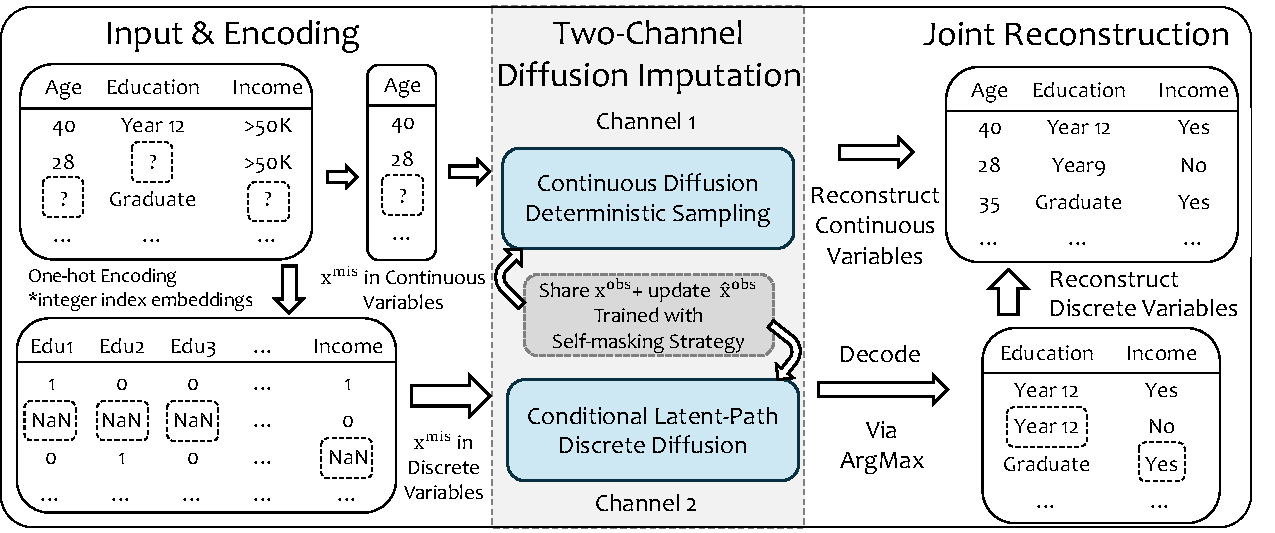
\includegraphics[width=\linewidth, height=0.24\textheight, keepaspectratio]{hdd.pdf}
\caption{
Overview of the \textbf{MissHDD} framework. Continuous and categorical
features are processed through two coordinated diffusion channels: a
conditional deterministic DDIM for continuous variables (Channel~1) and a
latent-path discrete diffusion model for categorical and other finite-state
variables (Channel~2). A self-masking strategy enables training
directly on incomplete data, and the outputs from both channels are merged to
produce the final imputed table.}
    \label{fig:MissHDD_overview}
\end{figure*}









\subsection{Channel 1: Conditional DDIM for Efficient Continuous Variable Imputation}

Continuous numerical features align naturally with Gaussian perturbations,
making diffusion models suitable for reconstructing missing numerical values.
However, standard DDPM sampling relies on long stochastic chains, which
introduce latency and variability that conflict with the stability and
reproducibility required for imputation. Deterministic DDIM~\cite{ddim,missddim} trajectories
address these limitations by replacing stochastic reverse transitions with
non-Markovian updates that preserve reconstruction quality while eliminating
sampling noise (see Figure~\ref{fig:ddim_wrap}). Building on this idea, MissHDD employs a conditional DDIM
formulation that reconstructs only the missing numerical coordinates while
conditioning all denoising steps on the observed ones.
\begin{wrapfigure}{r}{0.48\textwidth}
    \vspace{-10pt}
    \centering
    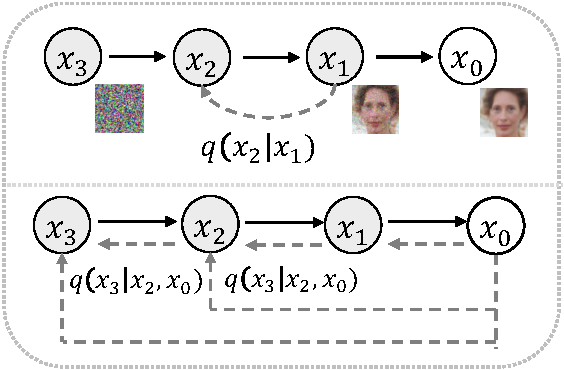
\includegraphics[width=0.47\textwidth]{plot.pdf} % <-- replace with your figure name
    \caption{
        Different sampling processes: traditional stochastic diffusion (top)
        versus deterministic non-Markovian inference (bottom).
    }
    \label{fig:ddim_wrap}
    \vspace{-10pt}
\end{wrapfigure}

\subsubsection{Forward diffusion on missing coordinates}
Let $\mathbf{x}_0^{\mathrm{mis}}$ denote the missing numerical components of
a sample. Only these coordinates are corrupted during the forward process:
\[
\mathbf{x}_t^{\mathrm{mis}}
= \sqrt{\alpha_t}\,\mathbf{x}_0^{\mathrm{mis}}
+ \sqrt{1-\alpha_t}\,\boldsymbol{\epsilon},
\] where $\boldsymbol{\epsilon}\sim\mathcal{N}(\mathbf{0},\mathbf{I})$
while observed numerical values remain fixed and are provided as conditioning
inputs. This formulation focuses the model on learning the conditional
distribution \(p(\mathbf{x}_0^{\mathrm{mis}} \mid \mathbf{x}_0^{\mathrm{obs}})\)
rather than the full joint distribution.

\subsubsection{Conditional reverse process}
A conditional noise-prediction network
$
\epsilon_\theta(\mathbf{x}_t^{\mathrm{mis}},\, t \mid \mathbf{x}_0^{\mathrm{obs}})
$
estimates the injected noise using both the corrupted missing coordinates and
the clean observed features. Under DDPM, the reverse transition would sample
from a Gaussian with variance $\sigma_t^2$, introducing stochasticity at each
step. In contrast, DDIM sets $\sigma_t=0$ and yields the deterministic update:
\begin{equation}
\mathbf{x}_{t-1}^{\mathrm{mis}}
=
\sqrt{\alpha_{t-1}}
\!\left(
\frac{\mathbf{x}_t^{\mathrm{mis}}
      - \sqrt{1-\alpha_t}\,
        \epsilon_\theta(\mathbf{x}_t^{\mathrm{mis}},t \mid \mathbf{x}_0^{\mathrm{obs}})}
     {\sqrt{\alpha_t}}
\right)
+
\sqrt{1-\alpha_{t-1}}\,
\epsilon_\theta(\mathbf{x}_t^{\mathrm{mis}},t\mid\mathbf{x}_0^{\mathrm{obs}}),
\end{equation}
producing stable and reproducible reconstructions while enabling large
timestep skips and faster inference.

\subsubsection{Training objective}
Following the DDPM/DDIM paradigm, the continuous channel is trained using a
conditional denoising score-matching objective:
\begin{equation}
\min_\theta
\mathbb{E}_{\mathbf{x}_0,\, t,\, \boldsymbol{\epsilon}}
\left[
\left\|
\boldsymbol{\epsilon}
-
\epsilon_\theta(\mathbf{x}_t^{\mathrm{mis}},\, t \mid \mathbf{x}_0^{\mathrm{obs}})
\right\|_2^2
\right],
\end{equation}
where only the missing numerical coordinates are noised and observed features
are supplied as conditioning inputs. This training procedure enables the
deterministic DDIM sampler to map $\mathbf{x}_T^{\mathrm{mis}}$ back to
$\mathbf{x}_0^{\mathrm{mis}}$ efficiently and with high stability.

% \subsection{Channel 1: Conditional DDIM for Efficient Continuous Variable Imputation}

% Numerical features in tabular data lie on a continuous Euclidean manifold where Gaussian noise
% and linear diffusion dynamics are well defined. This makes diffusion models a natural choice for
% learning conditional distributions over missing numerical values. However, standard
% Denoising Diffusion Probabilistic Models (DDPMs)~\cite{ddpm} employ a stochastic Markovian
% reverse process that requires hundreds of iterative denoising steps and injects randomness at each
% transition. While such stochasticity is beneficial for diverse generative sampling, it is fundamentally
% misaligned with the requirements of imputation, where outputs should be more efficient and stable. These limitations motivated the deterministic formulation introduced in DDIM~\cite{ddim}, and further demonstrated in our prior MissDDIM framework~\cite{missddim}, where we showed that
% deterministic non-Markovian trajectories provide accurate and low-variance imputations for continuous tabular data. In MissHDD, we build upon these insights by extending DDIM to a \emph{conditional} diffusion
% mechanism that reconstructs missing numerical coordinates while conditioning every denoising step on the observed portion of the input.

% \subsubsection{Forward diffusion on missing coordinates}
% %Let $\mathbf{x}_0 \in \mathbb{R}^d$ be a tabular sample and $\mathbf{m} \in \{0,1\}^d$ the
% %missingness mask. We decompose the sample into observed and missing subsets:
% %\[
% %\mathbf{x}_0^{\mathrm{obs}}=\mathbf{x}_0 \odot (1-\mathbf{m}), \qquad
% %\mathbf{x}_0^{\mathrm{mis}}=\mathbf{x}_0 \odot \mathbf{m}.
% %\]
% In the continuous channel, we operate only on the numerical coordinates within the
% missing subset $\mathbf{x}_0^{\mathrm{mis}}$ of $\mathbf{x}_0$; $\mathbf{x}_0^{\mathrm{mis,cont}}
% = \{ x_i : i \in \mathcal{I}_{\mathrm{mis}} \cap \mathcal{I}_{\mathrm{cont}} \}$. For notational simplicity, we denote this subset simply by
% $\mathbf{x}^{\mathrm{mis}}$. 
% Forward diffusion is applied only to the missing numerical dimensions, leaving
% observed features untouched. The corrupted latent state at step $t$ is:
% \[
% \mathbf{x}_t^{\mathrm{mis}} =
% \sqrt{\alpha_t}\,\mathbf{x}_0^{\mathrm{mis}}
% +\sqrt{1-\alpha_t}\,\boldsymbol{\epsilon},\qquad
% \boldsymbol{\epsilon}\sim\mathcal{N}(\mathbf{0},\mathbf{I}),
% \]
% where $\alpha_t=\prod_{s=1}^t(1-\beta_s)$ follows the variance schedule. This design allows the
% model to explicitly learn the conditional distribution
% \(
% p(\mathbf{x}_0^{\mathrm{mis}} \mid \mathbf{x}_0^{\mathrm{obs}}),
% \)
% rather than modeling the full joint distribution of heterogeneous tabular data.

% \subsubsection{Conditional reverse process.}
% To recover the missing components, this channel employs a conditional noise estimator:
% \[
% \epsilon_\theta(\mathbf{x}_t^{\mathrm{mis}},t\mid\mathbf{x}_0^{\mathrm{obs}}),
% \]
% which receives both the corrupted missing coordinates and the clean observed features. Under
% DDPM, the reverse transition is defined as a Gaussian:
% \[
% p_\theta(\mathbf{x}_{t-1}^{\mathrm{mis}}\mid\mathbf{x}_t^{\mathrm{mis}},\mathbf{x}_0^{\mathrm{obs}})
% =
% \mathcal{N}\!\left(
% \mathbf{x}_{t-1}^{\mathrm{mis}};\,
% \boldsymbol{\mu}_\theta(\mathbf{x}_t^{\mathrm{mis}},t\mid\mathbf{x}_0^{\mathrm{obs}}),\,
% \sigma_\theta^2(t)\mathbf{I}
% \right),
% \]
% with mean
% \[
% \boldsymbol{\mu}_\theta =
% \frac{1}{\sqrt{\alpha_t}}
% \left(
% \mathbf{x}_t^{\mathrm{mis}}
% -\frac{\beta_t}{\sqrt{1-\alpha_t}}\,
% \epsilon_\theta(\mathbf{x}_t^{\mathrm{mis}},t\mid\mathbf{x}_0^{\mathrm{obs}})
% \right).
% \]
% Because $\sigma_t>0$ under DDPM, each transition injects fresh Gaussian noise, producing
% irreducible sampling variance and slow convergence, two characteristics that contradict the
% requirements of tabular imputation.

% \subsubsection{Deterministic DDIM trajectories}
% DDIM introduces a family of non-Markovian reverse-time trajectories that remain \emph{consistent}
% with the objective optimized during DDPM training. Formally, DDIM reinterprets the DDPM reverse
% process as a discretization of an underlying generative ODE. Among the family of admissible
% solutions, setting the stochasticity parameter $\sigma_t=0$ yields a deterministic trajectory:
% \[
% \mathbf{x}_{t-1}^{\mathrm{mis}} =
% \sqrt{\alpha_{t-1}}
% \left(
% \frac{\mathbf{x}_t^{\mathrm{mis}}
%       -\sqrt{1-\alpha_t}\,
%        \epsilon_\theta(\mathbf{x}_t^{\mathrm{mis}},t\mid\mathbf{x}_0^{\mathrm{obs}})}
%      {\sqrt{\alpha_t}}
% \right)
% +
% \sqrt{1-\alpha_{t-1}}\,\epsilon_\theta(\mathbf{x}_t^{\mathrm{mis}},t\mid\mathbf{x}_0^{\mathrm{obs}}).
% \]
% This update eliminates all stochastic sampling noise while preserving the DDPM training objective,
% because DDIM trajectories correspond to exact solutions of the reverse-time ODE implied by the
% score model. A key consequence of adopting DDIM sampling is that the reverse mapping 
% $\mathbf{x}_T^{\mathrm{mis}} \rightarrow \mathbf{x}_0^{\mathrm{mis}}$ becomes fully deterministic, 
% yielding imputations that are stable and reproducible across runs. Moreover, DDIM supports large 
% non-uniform timestep skips (often 20-50 steps)~\cite{missddim} without compromising reconstruction quality, reducing sampling cost by an order of magnitude compared with DDPM. Finally, the absence of stochastic noise in the reverse trajectory eliminates variance accumulation, producing smoother and 
% more numerically stable denoising paths these properties which are particularly important for reliable 
% downstream inference and decision-making tasks.

% \subsubsection{Training objective.}
% The continuous channel of MissHDD follows the standard DDPM/DDIM training paradigm, 
% adapted to the conditional imputation setting. Given a sample with observed numerical 
% features $\mathbf{x}_0^{\mathrm{obs}}$ and missing targets $\mathbf{x}_0^{\mathrm{mis}}$, only the missing 
% coordinates are corrupted by the forward diffusion process:
% \[
% \mathbf{x}_t^{\mathrm{mis}}
% = \sqrt{\alpha_t}\,\mathbf{x}_0^{\mathrm{mis}}
%   + \sqrt{1-\alpha_t}\,\boldsymbol{\epsilon},
% \qquad 
% \boldsymbol{\epsilon}\sim\mathcal{N}(\mathbf{0},\mathbf{I}),
% \]
% while the observed entries remain fixed and are supplied as conditioning information 
% throughout the reverse steps.

% A conditional noise-prediction network
% \[
% \epsilon_\theta(\mathbf{x}_t^{\mathrm{mis}},\, t \mid \mathbf{x}_0^{\mathrm{obs}})
% \]
% is trained to recover the injected Gaussian noise. This leads to the conditional 
% denoising score-matching objective:
% \[
% \min_{\theta}\;
% \mathbb{E}_{\mathbf{x}_0,\, t,\, \boldsymbol{\epsilon}}
% \left[
% \left\|
% \boldsymbol{\epsilon}
% -
% \epsilon_\theta(\mathbf{x}_t^{\mathrm{mis}},\, t \mid \mathbf{x}_0^{\mathrm{obs}})
% \right\|_2^2
% \right],
% \]
% where $t$ is sampled uniformly from $\{1,\dots,T\}$.  
% This formulation trains the model to approximate the conditional score of the missing 
% components, enabling the deterministic DDIM sampler to reconstruct 
% $\mathbf{x}_0^{\mathrm{mis}}$ from $\mathbf{x}_T^{\mathrm{mis}}$ in a stable, efficient, and reproducible manner.

% \subsubsection{Limitations for categorical and discrete variables}

% Although DDIM offers an efficient and stable mechanism for continuous numerical features, its 
% formulation is fundamentally misaligned with the nature of categorical and other discrete 
% variables. Categorical values reside on a finite, unordered state space where Gaussian 
% perturbations and linear interpolation have no semantic meaning. As soon as the DDIM forward 
% step $\mathbf{x}_t=\sqrt{\alpha_t}\mathbf{x}_0+\sqrt{1-\alpha_t}\,\boldsymbol{\epsilon}$ is applied, 
% a one-hot vector or index embedding is mapped to a dense point in $\mathbb{R}^K$ that no longer 
% corresponds to any valid category, removing the sample from the discrete manifold at the very 
% first timestep.

% Because these intermediate noisy states are not legitimate categories, the reverse process becomes 
% ill-defined: the model must project ambiguous continuous vectors back onto a discrete set without 
% a meaningful geometric structure to guide the mapping. This often results in semantic drift, 
% collapsing class boundaries, and unstable denoising dynamics—well-documented failure modes of 
% continuous diffusion when applied to discrete domains. Moreover, DDIM relies on deterministic 
% ODE-based trajectories, which inherently assume a continuous underlying space; such trajectories 
% do not exist on discontinuous categorical manifolds without imposing continuous relaxations that 
% weaken categorical fidelity.

% These structural incompatibilities make continuous Gaussian diffusion unsuitable for discrete 
% variables. Effective imputation in this setting requires a diffusion process defined directly on 
% discrete probability simplexes, where transitions and denoising dynamics remain within the valid 
% state space.

% This motivates the second core component of MissHDD: a loopholing-based discrete diffusion 
% channel designed to model categorical and discrete variables natively. In the next section, we 
% describe how this discrete channel complements the continuous DDIM pathway to form a unified 
% heterogeneous imputation framework.


\subsubsection{Limitations for categorical and discrete variables}

Although DDIM provides an effective mechanism for continuous numerical
imputation, its Gaussian perturbations are incompatible with categorical and
other discrete variables. A one-hot vector or index embedding is mapped to a
dense continuous point immediately after the forward step
\(
\mathbf{x}_t=\sqrt{\alpha_t}\mathbf{x}_0+\sqrt{1-\alpha_t}\,\boldsymbol{\epsilon},
\)
placing the sample outside its valid discrete domain. The reverse process
must therefore recover categorical states from continuous intermediates that
carry no meaningful discrete structure, often leading to unstable updates
and loss of categorical consistency. As a result, continuous diffusion cannot
reliably model discrete variables without resorting to continuous
relaxations that compromise fidelity.

These limitations motivate the second component of MissHDD: a discrete
diffusion channel that operates directly within the probability domain of
categorical and other finite-state variables. The next section introduces
this discrete latent-path mechanism and its integration with the continuous
DDIM pathway.



% \subsection{Channel 2: Conditional Loopholing Diffusion for Categorical and Discrete Variables}

% While the continuous DDIM channel provides an efficient mechanism for imputing numerical
% features, categorical and other discrete variables require a fundamentally different generative
% process. As discussed earlier, Gaussian perturbations, linear interpolation, and continuous ODE
% trajectories are incompatible with discrete state spaces: a single diffusion step already pushes a
% categorical value off its valid manifold, making the reverse denoising process ill-posed.
% Accordingly, the second component of MissHDD adopts a \emph{loopholing-based discrete diffusion}
% framework~\cite{loopholing}, which was originally proposed for unconditional discrete generation.
% Loopholing diffusion defines its forward and reverse transitions directly on discrete probability
% simplexes, ensuring that all intermediate states remain valid categorical distributions and avoiding
% the probability–mass collapse commonly observed in one-hot diffusion. In MissHDD, we extend this framework to a \emph{conditional} form tailored to tabular imputation: the reverse denoising updates are conditioned on the observed features, and the forward corruption is applied only to the missing categorical coordinates. This conditional adaptation aligns the loopholing mechanism with the imputation objective, enabling coherent conditioning across timesteps and producing stable, semantically consistent reconstructions for categorical and discrete variables.


% Each sample from the discrete subset takes the form
% \[
% \mathbf{x}_0 \in \{1,\ldots,K_1\}\times\cdots\times\{1,\ldots,K_{d_{\mathrm{cat}}}\},
% \] with a corresponding mask $\mathbf{m}$ indicating which discrete coordinates require imputation. For each variable $x_j$, the model internally supports two equivalent representations: a one-hot vector $\mathbf{e}_{x_j} \in \{0,1\}^{K_j}$, or an integer index passed through a learnable embedding matrix. Both formats are naturally integrated in the proposed framework because loopholing diffusion operates over probability simplexes rather than Euclidean coordinates, allowing categorical distributions to be manipulated directly without continuous relaxations. In the discrete channel, we operate only on the categorical/discrete coordinates within the
% missing subset. Let $\mathbf{x}_0^{\mathrm{mis,cat}}
% = \{ x_i : i \in \mathcal{I}_{\mathrm{mis}} \cap \mathcal{I}_{\mathrm{cat}} \}$. 
% For notational simplicity, we denote this subset simply by
% $\mathbf{x}^{\mathrm{mis}}$.



% \subsubsection{Forward Process: Loopholing Corruption on categorical and discrete Simplexes.}
% For each missing categorical and discrete coordinate, the forward diffusion step transforms the one-hot 
% representation into a smoothed categorical and discrete distribution. Specifically, denote the categorical and discrete state 
% at time $t$ as a simplex vector $\mathbf{p}_t^{(j)} \in \Delta^{K_j-1}$. The forward kernel is defined as
% \begin{equation}
% q(\mathbf{p}_{t}^{(j)} \mid \mathbf{p}_{t-1}^{(j)})
% =(1-\beta_t)\mathbf{p}_{t-1}^{(j)}+\beta_t \mathbf{u}^{(j)},
% \label{eq:forward_cat}
% \end{equation}
% where $\mathbf{u}^{(j)}$ is the uniform distribution over categories. This loopholing mechanism 
% keeps $\mathbf{p}_t^{(j)}$ inside the simplex at all times, avoids invalid continuous vectors, and 
% ensures that the transition preserves class boundaries. For observed categories, the state is kept 
% fixed and supplied as a conditional context.

% \subsubsection{Conditional Reverse Process.}
% Given corrupted categorical and discrete distributions $\mathbf{p}_t^{\mathrm{mis}}$, the reverse process predicts the 
% clean categorical and discrete distribution at step $t-1$ using a conditional classifier $f_\theta(\mathbf{p}_t^{\mathrm{mis}}, t \mid \mathbf{x}^{\mathrm{obs}})$, which outputs logits corresponding to categorical and discrete transitions. The reverse kernel adopts the 
% loopholing form:
% \begin{equation}
% p_\theta(\mathbf{p}_{t-1}^{(j)} \mid \mathbf{p}_t^{(j)}, \mathbf{x}^{\mathrm{obs}})
% \propto
% \exp\!\left(
% f_\theta^{(j)}(\mathbf{p}_t^{(j)}, t \mid \mathbf{x}^{\mathrm{obs}})
% \right)
% \odot
% \left((1-\beta_t)\mathbf{p}_t^{(j)}+\beta_t\mathbf{u}^{(j)} \right),
% \label{eq:reverse_cat}
% \end{equation}
% where $\odot$ denotes elementwise multiplication. This structure ensures that the predicted reverse-time distribution remains entirely within the
% categorical and discrete simplex, faithfully mirrors the form of the forward transition kernel, and naturally incorporates observed features as conditioning signals. At the final step ($t=0$), the model produces a valid discrete output by selecting the most probable category for each variable
% via an $\arg\max$ operation.

% Loopholing diffusion is well-suited to categorical and discrete imputation because its transitions are defined directly on the probability simplex, ensuring that all intermediate states remain valid categorical distributions. This manifold preservation prevents the semantic drift typically observed
% when continuous diffusion is applied to discrete variables, allowing class boundaries to remain well defined throughout the trajectory. Moreover, the reverse denoising steps can incorporate the observed features as conditioning signals without relying on continuous relaxations or surrogate
% Gaussian noise. Importantly, the framework treats both one-hot and index-based embeddings consistently, as both representations are mapped to the same simplex space prior to diffusion, yielding a unified and structurally coherent approach to discrete imputation.


% \subsubsection{Training Objective.}
% The model is trained using a standard cross-entropy denoising objective:
% \begin{equation}
% \min_{\theta} 
% \mathbb{E}_{\mathbf{x}_0, t}
% \Big[
% \mathrm{CE}\big(
% \mathbf{p}_0^{\mathrm{mis}},
% f_\theta(\mathbf{p}_t^{\mathrm{mis}}, t \mid \mathbf{x}^{\mathrm{obs}})
% \big)
% \Big],
% \end{equation}
% where $\mathbf{p}_0^{\mathrm{mis}}$ is the ground-truth one-hot distribution for missing categories.

% Through this conditional loopholing diffusion mechanism, Channel 2 enables MissHDD to perform 
% categorical and discrete imputation in a manner that preserves discrete structure, avoids invalid continuous 
% states, and complements the efficient numerical imputation provided by the continuous DDIM channel.

\subsection{Channel 2: Conditional Latent-Path Discrete Diffusion (LPDD) for Categorical and Discrete Variables}


While the continuous DDIM channel handles numerical features effectively,
categorical and other discrete variables require a different generative
mechanism. To preserve discrete structure throughout diffusion, MissHDD
introduces a \emph{Latent-Path Discrete Diffusion (LPDD)} channel. LPDD is
inspired by the information-preserving pathway proposed in loopholing
diffusion~\cite{loopholing}, but is adapted to the feature-wise categorical
setting in tabular data and extended to a conditional form suitable for
imputation. Unlike continuous Gaussian diffusion, LPDD defines its forward
and reverse transitions directly on probability simplexes, ensuring that all
intermediate states remain valid categorical distributions and enabling
stable structure-preserving imputation for discrete variables.

\begin{wrapfigure}{r}{0.48\textwidth}
    \vspace{-10pt}
    \centering
    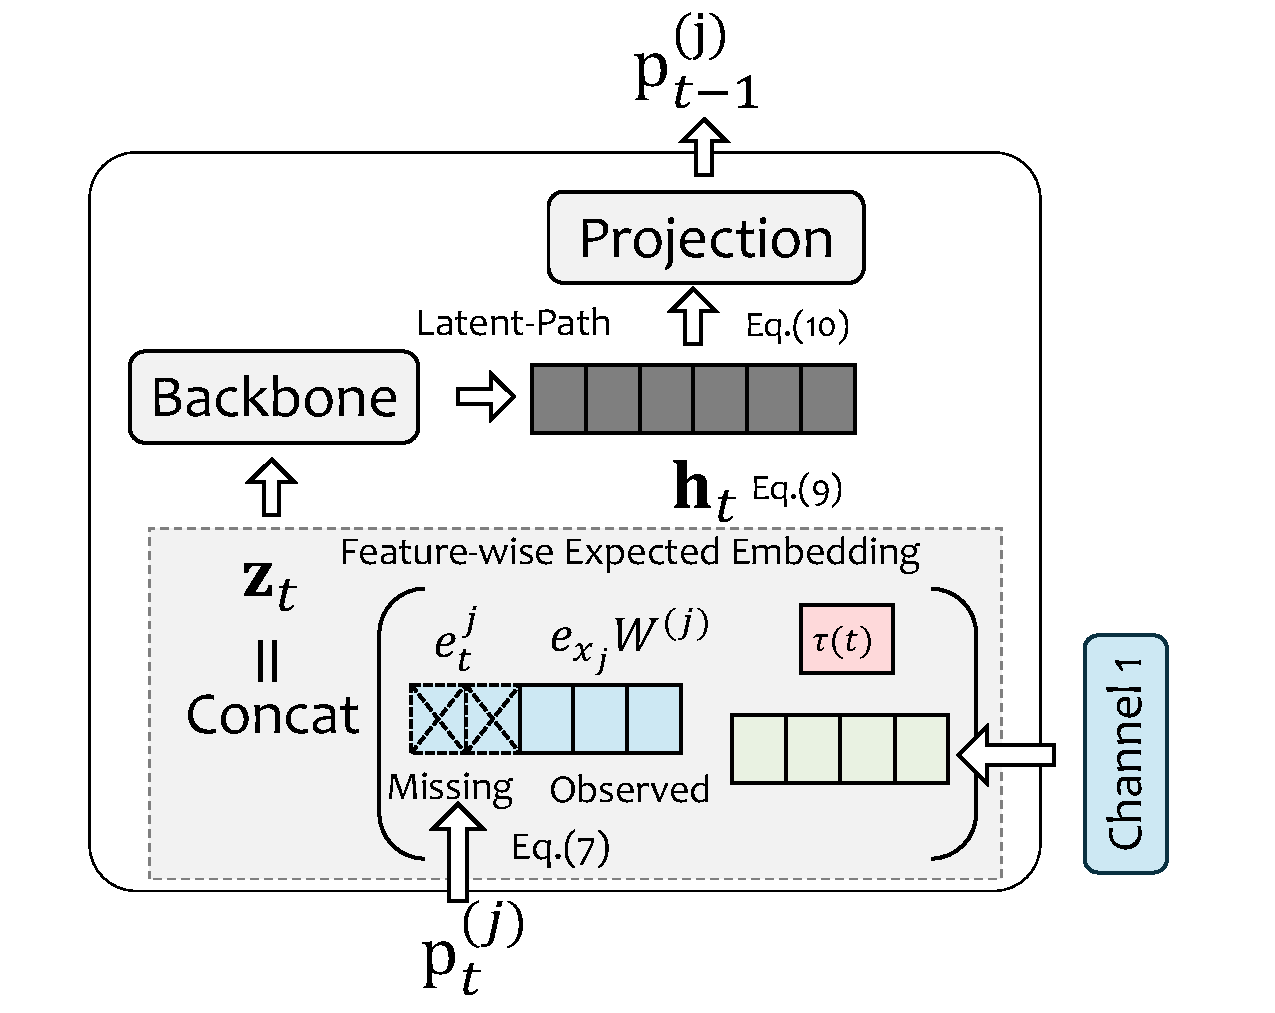
\includegraphics[width=0.47\textwidth]{c2.pdf} % <-- replace with your file c2.pdf
    \caption{
Overview of the LPDD reverse update at timestep $t$.
    }
    \label{fig:lpdd_overview}
    \vspace{-10pt}
\end{wrapfigure}



\subsubsection{Feature-wise representation and latent-path embedding}

Categorical features in tabular data differ widely in semantics and vocabulary
size. LPDD therefore models each categorical feature $j$ on its own probability
simplex $\Delta^{K_j-1}$ with vocabulary $V_j=\{1,\dots,K_j\}$. At diffusion
step $t$, the state of a missing categorical variable is represented as a
simplex vector $\mathbf{p}_t^{(j)}$, while an observed value is represented by
its one-hot vector $\mathbf{e}_{x_j}$. Thus observed categorical variables
remain fixed conditioning anchors, whereas missing categorical variables
evolve as simplex-valued distributions throughout the reverse trajectory.

\paragraph{Feature-wise expected embeddings}
To process categorical variables jointly with numerical features, every
categorical feature $j$ is equipped with a learnable embedding matrix
$W^{(j)}\in\mathbb{R}^{K_j\times d_h}$. At step $t$, we compute

\begin{equation}
\text{Observed:}\;\; \mathbf{e}_{x_j}W^{(j)}, \qquad
    \text{Missing:}\;\; \mathbf{e}^{(j)}_t = \mathbf{p}_t^{(j)}W^{(j)}.
\end{equation}


This expected embedding provides a continuous representation that preserves
feature semantics while ensuring compatibility with the backbone network.
Importantly, it allows LPDD to operate over probability distributions rather
than relaxed continuous states.

\paragraph{Conditional latent-path context}
The LPDD channel is a conditional adaptation of the Loopholing idea. Instead
of propagating only sampled categorical states, LPDD propagates distributional
information through expected embeddings and recomputes a latent pathway at
each reverse step using the observed context. Specifically, all categorical
embeddings, the latest numerical estimates from Channel~1, observed-value
indicators, missingness mask embeddings, and a time embedding $\tau(t)$ are
combined to form a unified contextual input

\begin{equation}
\mathbf{z}_t =
\mathrm{Concat}\!\left(
\{\mathbf{e}^{(j)}_t\}_{j\in\mathcal{I}_{\mathrm{cat}}},
\mathbf{x}^{\mathrm{cont}}_t,
\mathbf{m},
\tau(t)
\right),
\end{equation}

where $\mathbf{m}$ denotes the observed/missing indicator used by both
channels. The context $\mathbf{z}_t$ is passed through a shared feature
encoder to produce a latent hidden state:

\begin{equation}
\mathbf{h}_t = f_{\theta}^{\mathrm{backbone}}(\mathbf{z}_t).
\label{eq:project}
\end{equation}

\paragraph{Latent-path role of $\mathbf{h}_t$}
In LPDD, $\mathbf{h}_t$ serves as the \emph{latent path} that carries
conditional information across timesteps. Unlike the discrete state
$\mathbf{p}_t^{(j)}$, which is repeatedly corrupted toward a uniform
distribution, the latent state $\mathbf{h}_t$ preserves the current
distributional information, observed categorical anchors, numerical-channel
estimates, and the missingness pattern. This is the tabular conditional
counterpart of the Loopholing mechanism: the model avoids collapsing
intermediate categorical uncertainty into sampled one-hot states and instead
uses the latent pathway to guide the next simplex update.

This separation between the \emph{discrete path} $\mathbf{p}_t$ and the
\emph{continuous latent path} $\mathbf{h}_t$ is central to LPDD. It also
clarifies the conditioning mechanism: the categorical reverse transition is
not independent of the rest of the row, but is conditioned on observed
features, the mask, and the latest continuous-channel estimates at every
reverse diffusion step.


% \subsubsection{Forward diffusion: simplex-preserving corruption}
% For each missing categorical variable, loopholing diffusion performs a
% simplex-preserving interpolation between the clean one-hot distribution and a
% uniform prior:

% \[
% \mathbf{p}_{t}^{(j)}
% = (1-\beta_t)\mathbf{p}_{t-1}^{(j)} + \beta_t \mathbf{u}^{(j)},
% \]

% where $\mathbf{u}^{(j)}$ is uniform over $V_j$. This transition keeps
% $\mathbf{p}_t^{(j)}$ strictly inside $\Delta^{K_j-1}$, preventing invalid
% continuous states and allowing clean categorical distributions to degrade in a
% controlled manner. Observed variables remain fixed and serve as conditioning
% anchors throughout diffusion.

% \subsubsection{Forward diffusion: simplex-preserving corruption}

% For each missing categorical variable, LPDD performs a simplex-preserving
% interpolation that gradually moves a clean one-hot distribution toward a
% uniform prior. For feature $j$, the forward transition is

% \[
% \mathbf{p}_{t}^{(j)}
% = (1-\beta_t)\,\mathbf{p}_{t-1}^{(j)} + \beta_t\,\mathbf{u}^{(j)},
% \]

% where $\mathbf{u}^{(j)}$ is the uniform distribution over the vocabulary
% $V_j$. This update keeps $\mathbf{p}_{t}^{(j)}$ strictly inside the
% probability simplex $\Delta^{K_j-1}$ for all $t$, allowing categorical states
% to degrade smoothly without leaving their valid domain. Observed categorical
% values remain fixed and act as conditioning anchors throughout diffusion.

% \subsubsection{Conditional reverse process}

% Given corrupted categorical states $\mathbf{p}_t^{\mathrm{mis}}$, the backbone
% produces feature-wise logits

% \[
% f_\theta^{(j)}(\mathbf{p}_t^{(j)},t\mid\mathbf{x}^{\mathrm{obs}})\in\mathbb{R}^{K_j}.
% \]

% LPDD mirrors the form of the forward kernel to construct a simplex-consistent
% reverse transition:

% \[
% p_\theta(\mathbf{p}_{t-1}^{(j)} \mid \mathbf{p}_t^{(j)}, \mathbf{x}^{\mathrm{obs}})
% \propto
% \exp\!\left(f_\theta^{(j)}(\mathbf{p}_t^{(j)},t\mid\mathbf{x}^{\mathrm{obs}})\right)
% \odot
% \Big((1-\beta_t)\mathbf{p}_t^{(j)} + \beta_t\,\mathbf{u}^{(j)}\Big),
% \]

% followed by normalization. This latent-path update:

% 1. preserves the simplex constraint at every timestep;  
% 2. incorporates observed categorical features as conditional guidance through the backbone;  
% 3. ensures reverse denoising remains aligned with the semantics of the forward corruption.

% At $t=0$, the model produces a discrete imputation via

% \[
% x^{(j)}_{\text{imp}}=\arg\max_k [\mathbf{p}_0^{(j)}]_k.
% \]

% \subsubsection{Training objective}

% Training focuses only on missing categorical coordinates. Given ground-truth
% one-hot targets $\mathbf{p}_0^{\mathrm{mis}}$, LPDD uses a conditional
% cross-entropy denoising objective:

% \[
% \min_\theta\;
% \mathbb{E}_{\mathbf{x}_0,t}\;
% \mathrm{CE}\!\left(
% \mathbf{p}_0^{\mathrm{mis}},\;
% f_\theta(\mathbf{p}_t^{\mathrm{mis}},t\mid\mathbf{x}^{\mathrm{obs}})
% \right).
% \]

% This objective learns a conditional discrete score directly on the probability
% domain, enabling stable and structure-preserving reconstruction of categorical
% variables.

% Together with the deterministic DDIM channel for numerical features, LPDD
% provides a principled discrete counterpart that maintains categorical validity
% throughout diffusion, yielding a unified heterogeneous diffusion framework for
% mixed-type tabular imputation.

\subsubsection{Forward diffusion: simplex-preserving corruption}

For each missing categorical variable, LPDD performs a simplex-preserving
interpolation that gradually moves a clean one-hot distribution toward a
uniform prior. For feature $j$, the forward transition is

\[
\mathbf{p}_{t}^{(j)}
= (1-\beta_t)\,\mathbf{p}_{t-1}^{(j)} + \beta_t\,\mathbf{u}^{(j)},
\]

where $\mathbf{u}^{(j)}$ is the uniform distribution over the vocabulary
$V_j$. This update keeps $\mathbf{p}_{t}^{(j)}$ strictly inside the
probability simplex $\Delta^{K_j-1}$ for all $t$, allowing categorical states
to degrade smoothly without leaving their valid domain. Observed categorical
values remain fixed and act as conditioning anchors throughout diffusion.


\subsubsection{Conditional reverse process}

Given the corrupted categorical states $\mathbf{p}_t^{\mathrm{mis}}$, we first
form the contextual representation $\mathbf{z}_t$ and latent-path state
(Eq.\ref{eq:project}) as described
above. A feature-wise projection head then maps $\mathbf{h}_t$ to logits for
each categorical variable:
\begin{equation}
\boldsymbol{\ell}_t^{(j)} = g_\theta^{(j)}(\mathbf{h}_t)
\in \mathbb{R}^{K_j}.
\label{eq:project10}
\end{equation}

LPDD mirrors the form of the forward kernel to construct a
simplex-consistent reverse transition. For feature $j$, the unnormalised
reverse update is
\begin{equation}
\tilde{\mathbf{p}}_{t-1}^{(j)} =
\exp\!\big(\boldsymbol{\ell}_t^{(j)}\big)
\odot
\Big((1-\beta_t)\,\mathbf{p}_t^{(j)} + \beta_t\,\mathbf{u}^{(j)}\Big),
\label{eq:lpdd_unnormalized}
\end{equation}
and the normalized reverse state is
\begin{equation}
\mathbf{p}_{t-1}^{(j)}
=
\Pi_{\Delta}\!\left(\tilde{\mathbf{p}}_{t-1}^{(j)}\right)
=
\frac{\tilde{\mathbf{p}}_{t-1}^{(j)}+\varepsilon}
{\left\|\tilde{\mathbf{p}}_{t-1}^{(j)}+\varepsilon\right\|_1},
\label{eq:lpdd_reverse}
\end{equation}
where $\Pi_{\Delta}$ denotes projection by positive normalization onto the
probability simplex, and $\varepsilon$ is a small numerical constant used to
avoid zero denominators. In other words, the forward kernel
\((1-\beta_t)\mathbf{p}_t^{(j)} + \beta_t\mathbf{u}^{(j)}\) defines how mass
can move within the simplex, while the logits $\boldsymbol{\ell}_t^{(j)}$
derived from $\mathbf{h}_t$ indicate where probability should
concentrate given the global context. This coupling makes the reverse update
depend jointly on the current simplex state $\mathbf{p}_t^{(j)}$ and the
latent path $\mathbf{h}_t$.

This update is deterministic once the network parameters and conditioning
context are fixed. It should therefore be interpreted as a conditional
simplex-valued denoising operator rather than as a stochastic categorical
sampling step. The simplex constraint follows directly from
Eq.~\eqref{eq:lpdd_reverse}: if $\mathbf{p}_t^{(j)}\in\Delta^{K_j-1}$ and
$\beta_t\in[0,1]$, then the forward-kernel term is non-negative; the
exponential logits are strictly positive; their elementwise product is
positive; and the $L_1$ normalization maps the result back to
$\Delta^{K_j-1}$. Thus LPDD preserves non-negativity and unit mass at every
reverse step, which prevents invalid categorical states during denoising.

At $t=0$, the model produces a discrete imputation via
\[
x^{(j)}_{\text{imp}} = \arg\max_k [\mathbf{p}_0^{(j)}]_k,
\]
which is a constant-time decoding step. Thus final categorical decoding adds
negligible cost relative to the reverse updates.



% \subsubsection{Conditional reverse process}

% Given corrupted categorical states $\mathbf{p}_t^{\mathrm{mis}}$, the backbone
% produces feature-wise logits

% \[
% f_\theta^{(j)}(\mathbf{p}_t^{(j)},t\mid\mathbf{x}^{\mathrm{obs}})\in\mathbb{R}^{K_j}.
% \]

% LPDD mirrors the form of the forward kernel to construct a simplex-consistent
% reverse transition:

% \begin{equation}
% p_\theta(\mathbf{p}_{t-1}^{(j)} \mid \mathbf{p}_t^{(j)}, \mathbf{x}^{\mathrm{obs}})
% \propto
% \exp\!\left(f_\theta^{(j)}(\mathbf{p}_t^{(j)},t\mid\mathbf{x}^{\mathrm{obs}})\right)
% \odot
% \Big((1-\beta_t)\mathbf{p}_t^{(j)} + \beta_t\,\mathbf{u}^{(j)}\Big)
% \end{equation}

% followed by normalization. This latent-path update preserves the simplex constraint at every timestep, incorporates observed categorical features as conditional guidance through the backbone and it also ensures reverse denoising remains aligned with the semantics of the forward corruption.

% At $t=0$, the model produces a discrete imputation via

% \[
% x^{(j)}_{\text{imp}}=\arg\max_k [\mathbf{p}_0^{(j)}]_k.
% \]

\subsubsection{Training Objective}

For the LPDD channel, only the categorical coordinates marked as missing
under the self-masking strategy contribute to the training loss. Let
$\mathbf{p}_0^{(j)}$ denote the ground-truth one-hot distribution of feature
$j$. At diffusion step $t$, the model first forms the contextual embedding
$\mathbf{z}_t$, computes the latent-path state (Eq.\ref{eq:project}), and then
produces feature-wise logits via the projection head (Eq.\ref{eq:project10}).

The LPDD training objective is a conditional cross-entropy denoising loss:

\begin{equation}
\min_{\theta}\;
\mathbb{E}_{\mathbf{x}_0,\, t}\;
\mathrm{CE}\!\left(
\mathbf{p}_0^{\mathrm{mis}},\;
\boldsymbol{\ell}_t^{\mathrm{mis}}
\right),
\end{equation}

where $\boldsymbol{\ell}_t^{\mathrm{mis}}$ collects the logits for all
categorical features designated as missing at training time. This objective
learns a conditional discrete score directly on the probability simplex,
enabling the reverse diffusion process to reconstruct categorical variables in
a stable and structure-preserving manner.

The complete MissHDD training objective combines the continuous DDIM loss and
the LPDD categorical loss:
\begin{equation}
\mathcal{L}_{\mathrm{MissHDD}}
=
\mathcal{L}_{\mathrm{cont}}
+
\lambda_{\mathrm{cat}}\mathcal{L}_{\mathrm{cat}},
\label{eq:joint_loss}
\end{equation}
where $\mathcal{L}_{\mathrm{cont}}$ is the conditional noise-prediction MSE
defined for missing numerical coordinates, $\mathcal{L}_{\mathrm{cat}}$ is the
cross-entropy loss above, and $\lambda_{\mathrm{cat}}$ balances the two
feature types. The two channels are trained jointly end-to-end. Gradients from
both losses update the shared contextual encoder, while the continuous noise
head and categorical projection heads receive their corresponding
type-specific gradients.


% Together with the deterministic DDIM channel for numerical features, LPDD
% provides a principled discrete counterpart that maintains categorical validity
% throughout diffusion, yielding a unified heterogeneous diffusion framework for
% mixed-type tabular imputation.

\begin{figure}[t]
    \centering
    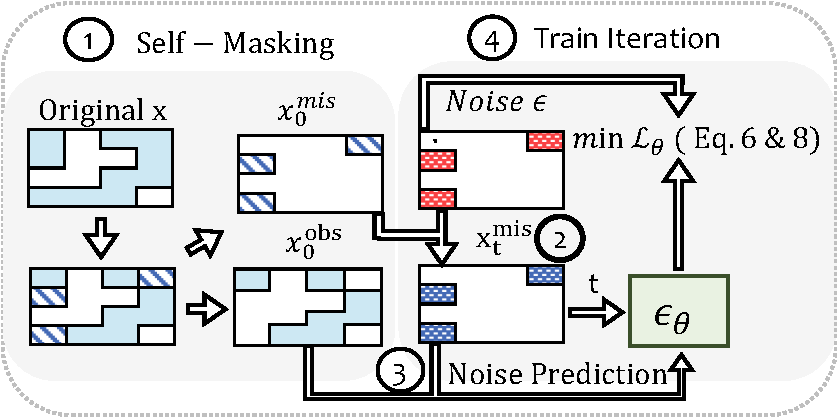
\includegraphics[width=0.8\linewidth]{missddim.pdf}
    \caption{
    Self-masking strategy used in MissHDD.  
    During training, a portion of observed entries is randomly masked to create 
    pseudo-missing targets. The remaining entries serve as conditioning information for 
    both the continuous and discrete diffusion channels.
    }
    \label{fig:fig_self_masking}
\end{figure}

\subsection{Self-masking Strategy for Incomplete Data}

Training generative models on incomplete tabular data is difficult because
only a subset of entries is observed, and preprocessing them with external
imputers (e.g., mean filling~\cite{mean} or K-NN~\cite{knn} method) introduces bias before the diffusion
model is learned. To avoid such artifacts, MissHDD adopts a \textbf{self-masking}
strategy that enables both diffusion channels to learn directly from partially
observed samples.

For each training input, the original missingness pattern is preserved to
respect the true underlying mechanism. Additionally, a small random subset of
the observed entries is temporarily masked to create pseudo-missing targets,
while the remaining observed values are used as conditioning information.
Formally, letting $\mathbf{m}$ denote the original mask and $\tilde{\mathbf{m}}$
the auxiliary random mask, the effective training mask becomes
$
\mathbf{m}_{\mathrm{train}} = \mathbf{m} \;\lor\; \tilde{\mathbf{m}},
$
so that pseudo-missing entries are treated in the same way as true missing
values during both the forward and reverse diffusion steps.

This procedure provides two benefits. First, it increases the amount of
supervised signal available for learning the conditional distribution
$p(\mathbf{x}_0^{\mathrm{mis}} \mid \mathbf{x}_0^{\mathrm{obs}})$ without
requiring fully observed samples. Second, it regularizes both the continuous
DDIM channel and the LPDD channel by exposing them to slightly perturbed
missingness patterns, improving robustness to realistic training conditions. Figure~\ref{fig:fig_self_masking} illustrates the process: the same
self-masked sample is passed to both diffusion channels, which reconstruct the
masked numerical and categorical entries jointly under a consistent
conditioning pattern.




\subsection{Joint Reconstruction}

The two diffusion channels in MissHDD do not operate independently. At every
reverse diffusion step $t$, both channels are conditioned on the same unified
contextual representation $\mathbf{z}_t$, which includes (i) the observed
features and (ii) the most recent estimates produced by the other channel.
This shared-conditioning design keeps numerical and categorical trajectories
aligned throughout the denoising process. During inference, the channels are
updated synchronously: the current continuous estimates and categorical
simplex states are first embedded into $\mathbf{z}_t$, the DDIM update is
applied to missing numerical coordinates, the LPDD update is applied to
missing categorical simplexes, and the updated states are then fed back into
the next reverse step. When $t=0$ is reached, the continuous DDIM channel outputs the deterministic
numerical reconstruction $\hat{\mathbf{x}}^{\mathrm{cont}}$, and the LPDD
channel yields categorical distributions whose MAP assignments form
$\hat{\mathbf{x}}^{\mathrm{cat}}$. The final imputed sample is obtained by $ \hat{\mathbf{x}} = \hat{\mathbf{x}}^{\mathrm{cont}}\cup \hat{\mathbf{x}}^{\mathrm{cat}},$ with the union respecting the original feature order. Because both channels evolve under the same conditioning signals, the result is a single coherent estimate of $p(\mathbf{x}^{\mathrm{mis}} \mid \mathbf{x}^{\mathrm{obs}})$ rather than two
independent imputations, ensuring that cross-type dependencies are preserved.

\begin{algorithm}[t]
\caption{MissHDD joint training with self-masking}
\label{alg:training}
\algsmall
\begin{algorithmic}[1]
\Require Mini-batch $\mathcal{B}=\{(\mathbf{x}_i,\mathbf{m}_i)\}$, self-mask ratio $\rho$, steps $T$
\Require Parameters $\theta=\{\theta_{\mathrm{sh}},\theta_{\mathrm{cont}},\theta_{\mathrm{cat}}\}$
\For{each mini-batch $\mathcal{B}$}
    \ForAll{$(\mathbf{x},\mathbf{m})\in\mathcal{B}$}
        \State $\tilde{\mathbf{m}}\sim\mathrm{Mask}(\mathbf{1}-\mathbf{m};\rho)$;\quad
        $\mathbf{m}_{\mathrm{train}}\gets \mathbf{m}\lor\tilde{\mathbf{m}}$;\quad
        $t\sim\mathrm{Uniform}(\{1,\ldots,T\})$
        \State $\mathbf{x}^{\mathrm{cont}}_t\gets q_{\mathrm{cont}}(\mathbf{x}^{\mathrm{cont}}_0,t,\mathbf{m}_{\mathrm{train}})$;\quad
        $\mathbf{p}^{\mathrm{cat}}_t\gets q_{\mathrm{cat}}(\mathbf{p}^{\mathrm{cat}}_0,t,\mathbf{m}_{\mathrm{train}})$
        \State $\mathbf{z}_t\gets f_{\theta_{\mathrm{sh}}}(\mathbf{x}^{\mathrm{obs}},\mathbf{m}_{\mathrm{train}},
        \mathbf{x}^{\mathrm{cont}}_t,\mathbf{p}^{\mathrm{cat}}_t,t)$
        \State $\hat{\boldsymbol{\epsilon}}\gets g_{\theta_{\mathrm{cont}}}(\mathbf{z}_t)$;\quad
        $\hat{\boldsymbol{\ell}}\gets h_{\theta_{\mathrm{cat}}}(\mathbf{z}_t)$
    \EndFor
    \State $\mathcal{L}\gets \mathcal{L}_{\mathrm{cont}}(\hat{\boldsymbol{\epsilon}},\boldsymbol{\epsilon})
    +\lambda_{\mathrm{cat}}\mathcal{L}_{\mathrm{cat}}(\hat{\boldsymbol{\ell}},\mathbf{p}^{\mathrm{cat}}_0)$
    \State $\theta\gets\mathrm{Adam}(\theta,\nabla_\theta\mathcal{L})$
\EndFor
\State \Return $\theta$
\end{algorithmic}
\end{algorithm}

\begin{algorithm}[t]
\caption{MissHDD deterministic inference}
\label{alg:inference}
\algsmall
\begin{algorithmic}[1]
\Require Incomplete input $\mathbf{x}^{\mathrm{obs}}$, mask $\mathbf{m}$, schedule $\tau_S>\cdots>\tau_0=0$
\State Initialize missing continuous entries with $\mathcal{N}(\mathbf{0},\mathbf{I})$ and missing categorical simplexes with $\mathbf{u}^{(j)}$
\For{$s=S,\ldots,1$}
    \State $\mathbf{z}_{\tau_s}\gets f_{\theta_{\mathrm{sh}}}(\mathbf{x}^{\mathrm{obs}},\mathbf{m},
    \mathbf{x}^{\mathrm{cont}}_{\tau_s},\mathbf{p}^{\mathrm{cat}}_{\tau_s},\tau_s)$
    \State $\mathbf{x}^{\mathrm{cont}}_{\tau_{s-1}}\gets
    \mathrm{DDIM}_{\eta=0}(\mathbf{x}^{\mathrm{cont}}_{\tau_s},g_{\theta_{\mathrm{cont}}}(\mathbf{z}_{\tau_s}))$
    \ForAll{missing categorical features $j$}
        \State $\boldsymbol{\ell}^{(j)}_{\tau_s}\gets h_{\theta_{\mathrm{cat}}}^{(j)}(\mathbf{z}_{\tau_s})$
        \State $\mathbf{p}^{(j)}_{\tau_{s-1}}\gets
        \Pi_\Delta\!\left(\exp(\boldsymbol{\ell}^{(j)}_{\tau_s})
        \odot\big((1-\beta_{\tau_s})\mathbf{p}^{(j)}_{\tau_s}+\beta_{\tau_s}\mathbf{u}^{(j)}\big)\right)$
    \EndFor
\EndFor
\State $\hat{x}^{(j)}_{\mathrm{cat}}\gets \arg\max_k[\mathbf{p}^{(j)}_{0}]_k$
\State \Return $\mathrm{Merge}(\mathbf{x}^{\mathrm{obs}},\mathbf{x}^{\mathrm{cont}}_0,\hat{\mathbf{x}}^{\mathrm{cat}},\mathbf{m})$
\end{algorithmic}
\end{algorithm}



\section{Experimental Setup}

We evaluate \texttt{MissHDD} by imputation accuracy, downstream task utility,
sampling efficiency, and stability.

% Code will be available at: \url{https://github.com/echoid/MissDDIM}

% % \subsection{Experimental Setup}
\subsection{Datasets}

We evaluate \texttt{MissHDD} on fourteen heterogeneous tabular datasets from
the UCI Machine Learning Repository\footnote{\url{https://archive.ics.uci.edu/}}
and Kaggle\footnote{\url{https://www.kaggle.com/}}. Table~\ref{tab:dataset_summary}
summarizes their sample sizes, feature types, labels, and missing rates.

We group our evaluation datasets into two categories:

\textbf{Category 1: Synthetic Missingness on Fully Observed Data.}
This category contains eight complete datasets with synthetic MCAR, MAR, and
MNAR masks, enabling controlled evaluation under known missingness mechanisms.

\textbf{Category 2: Naturally Incomplete Real-World Data.}
This category includes six originally incomplete datasets with unknown or mixed
missingness, reflecting practical data collection conditions.





\subsection{Synthetic Incomplete Data Generation}

We introduce synthetic \textbf{MCAR}, \textbf{MAR}, and \textbf{MNAR} masks at
30\%, 50\%, and 70\% missingness using \texttt{MissMecha}~\cite{missmecha},
with identical masks across all methods.

\paragraph*{MCAR}
Missingness is independent of both observed and unobserved variables, with
entries removed uniformly at random.

\paragraph*{MAR}
Missingness depends only on observed covariates. Certain feature values
condition the probability of removal in another feature, following the
standard MAR formulation.

\paragraph*{MNAR}
Missingness depends on the value of the feature being masked. Removal
probabilities increase for specific value ranges or categories, reflecting
self-dependent omission patterns commonly found in practice.



\begin{table}[t]
\caption{Benchmark datasets. Cate. and Cont. denote categorical and continuous
features; missing rates apply only to originally incomplete datasets.}
\label{tab:dataset_summary}
\centering
\resizebox{0.78\linewidth}{!}{%
\begin{tabular}{lrrrrr}
\toprule
\multicolumn{6}{c}{\textit{Category 1: Synthetic Missingness on Fully Observed Data}} \\
\midrule
\textbf{Dataset} & \textbf{Samples} & \textbf{Cate.} & \textbf{Cont.} & \textbf{Label} & \textbf{Missing Rate} \\
\midrule
Adult        & 48,842 & 7  & 7  & 2 classes      & — \\
Banknote     & 1,372  & 0  & 4  & 2 classes      & — \\
Breast       & 2,869  & 4  & 0  & 2 classes      & — \\
Letter       & 20,000 & 0  & 16 & 26 classes     & — \\
California   & 20,640 & 0  & 8  & Regression     & — \\
E-commerce   & 10,999 & 7  & 3  & Regression     & — \\
Student      &   649  & 11 & 2  & Regression     & — \\
Yacht        &   308  & 0  & 6  & Regression     & — \\
\midrule
\multicolumn{6}{c}{\textit{Category 2: Naturally Incomplete Real-World Data}} \\
\midrule
\textbf{Dataset} & \textbf{Samples} & \textbf{Cate.} & \textbf{Cont.} & \textbf{Label} & \textbf{Missing Rate} \\
\midrule
Hepat     & 155 & 13 & 6  & 2 classes  & 5.67\%  \\
Horse     & 368 & 14 & 8  & 2 classes  & 23.80\% \\
Kidney    & 400 & 12 & 12 & 2 classes  & 10.54\% \\
Mammo     & 961 & 4  & 1  & 2 classes  & 3.37\%  \\
Pima      & 768 & 0  & 8  & 2 classes  & 12.24\% \\
Wiscon    & 699 & 9  & 0  & 2 classes  & 0.25\%  \\
\bottomrule
\end{tabular}
}
\end{table}



\subsection{Baselines}

We compare \texttt{MissHDD} with statistical, deep generative, and
diffusion-based imputers.

\paragraph{Statistical Baselines}
We compare against classical imputers including \texttt{Mean/Mode}
substitution, \texttt{MICE}~\cite{mice}, and \texttt{MissForest}~\cite{missforest}.
These lightweight methods provide standard non-generative reference points.

\paragraph{Deep Generative Models}
We include two representative latent-variable models: \texttt{GAIN}~\cite{yoon2018gain},
a GAN-based imputer trained with adversarial learning, and \texttt{MIWAE}~\cite{mattei2019miwae},
a VAE-based method optimized with an importance-weighted objective.
Both capture nonlinear dependencies but rely on continuous or embedded
categorical representations.

\paragraph{Diffusion-based Models}
We evaluate three diffusion-based imputers: \texttt{CSDI}~\cite{csdi}, its
tabular extension \texttt{TabCSDI}~\cite{tabcsdi}, and \texttt{MissDiff}~\cite{missdiff}.
Diffusion baselines use their reported/default reverse schedules with 100
stochastic samples per instance, aggregated by the median. \texttt{MissHDD}
uses deterministic one-pass imputation through its continuous DDIM and LPDD
channels.


% \subsection{Evaluation Metrics}

% %\subsubsection{Imputation Error Metrics}

% Following established practice in heterogeneous tabular imputation, we evaluate the accuracy of imputation using the \textbf{Imputation Error (ImpErr)}, defined as:
% \[
% ImpErr(\mathbf{x}, \hat{\mathbf{x}}) = \sqrt{
% \frac{1}{d}\sum_{i \in \mathcal{I}_{\mathrm{cont}}} |\mathbf{x}_{i} - \hat{\mathbf{x}}_{i}|^{2} + \sum_{i \in \mathcal{I}_{\mathrm{cat}}} \mathbb{I}(\mathbf{x}_{i} \neq \hat{\mathbf{x}}_{i})^{2}}
% %\text{ImpErr} = \frac{1}{D} \sum_{d=1}^{D} \mathrm{err}(d),
% \]
% %where the per–feature error $\mathrm{err}(d)$ depends on the variable type.

% %\paragraph{Continuous variables}
% %For numerical features, we report the \textbf{ Root Mean Squared Error (RMSE)}:
% %\begin{equation}
% %\mathrm{err}(d)
% %= 
% %\sqrt{
% %\frac{1}{n_d}\sum_{i \in \mathcal{M}_d} (X_{id} - \hat{X}_{id})^{2}
% %}
% %\label{eq:nrmse}
% %\end{equation}

% %\paragraph{Categorical variables}
% %For discrete categorical features, reconstruction quality is measured by the
% %\textbf{accuracy error}:
% %\begin{equation}
% %\mathrm{err}(d)
% %=
% %\frac{1}{n_d}
% %\sum_{i \in \mathcal{M}_d}
% %\mathbb{I}(X_{id} \neq \hat{X}_{id}),
% %\label{eq:caterr}
% %\end{equation}
% %where $\hat{X}_{id} = \arg\max$ over the predicted categorical distribution.

% %\paragraph{Ordinal variables.}
% %If a categorical feature is ordinal with $R_d$ ordered levels, we additionally report the
% %\textbf{displacement error}:
% %\begin{equation}
% %\mathrm{err}(d)
% %=
% %\frac{1}{n_d}
% %\sum_{i \in \mathcal{M}_d}
% %\left|
% %\frac{X_{id} - \hat{X}_{id}}{R_d}
% %\right|.
% %\label{eq:orderr}
% %\end{equation}
% %This penalizes incorrect predictions proportionally to their ordinal distance.

% We also report a unified mixed-type imputation metric, the Mixed Imputation
% Error (ImpErr), which combines continuous and categorical errors with
% dimension-aware weights:
% \[
% w_{\text{cont}} = \frac{d_{\text{cont}}}{d}, \qquad
% w_{\text{cat}} = \frac{d_{\text{cat}}}{d},
% \]
% \[
% \mathrm{MixErr}
% =
% w_{\text{cont}} \cdot \mathrm{RMSE}_{\text{cont}}
% +
% w_{\text{cat}} \cdot \mathrm{CatErr}.
% \]
% This aggregation preserves the heterogeneous feature composition by weighting
% each error term according to its proportion of the total dimensionality,
% rather than imposing arbitrary equal weights.


% We also assessed the effectiveness of imputed complete data for downstream classification or regression tasks, depending on whether the target variable is discrete or continuous. We evaluated classifcation and regression performances in terms of F1-Score and Mean Average Error (MAE), respectively.


\subsection{Evaluation Metrics}

Because heterogeneous tabular data contain both continuous and categorical
features, we evaluate imputation quality using type-specific metrics and a
dimension-aware unified metric.

\paragraph{Continuous Imputation Error}
For continuous variables, imputation accuracy is measured using the Root
Mean Squared Error (RMSE) computed only over the masked entries:
\[
\mathrm{RMSE}
=
\sqrt{
\frac{1}{N_{\mathrm{cont}}^{\mathrm{mis}}}
\sum_{j=1}^{n}
\sum_{i \in \mathcal{I}_{\mathrm{cont}}}
M_{j,i}\,\big(x_{j,i} - \hat{x}_{j,i}\big)^{2}
},
\]
where \(M_{j,i}=1\) indicates that entry \((j,i)\) was masked and contributes
to the evaluation.

\paragraph{Categorical Imputation Error}
For categorical variables, we report the classification error over the masked
entries:
\[
\mathrm{CatErr}
=
\frac{1}{N_{\mathrm{cat}}^{\mathrm{mis}}}
\sum_{j=1}^{n}
\sum_{i \in \mathcal{I}_{\mathrm{cat}}}
M_{j,i}\,\mathbb{I}(x_{j,i} \neq \hat{x}_{j,i}),
\]
where \(\mathbb{I}(\cdot)\) is the indicator function.

\paragraph{ImpErr}
To aggregate continuous and categorical errors into a single measure while
preserving the heterogeneous dimensionality of the feature space, we define
the Mixed Imputation Error (ImpErr) as a dimension-weighted combination:
\[
w_{\mathrm{cont}} = \frac{d_{\mathrm{cont}}}{d},
\qquad
w_{\mathrm{cat}} = \frac{d_{\mathrm{cat}}}{d},
\]
\[
\mathrm{ImpErr}
=
w_{\mathrm{cont}} \cdot \mathrm{RMSE}_{\mathrm{cont}}
+
w_{\mathrm{cat}} \cdot \mathrm{CatErr}.
\]
This dimension-weighted metric reflects each dataset's continuous/categorical
composition. Since all features are normalized to \([0,1]\), lower ImpErr
indicates better mixed-type reconstruction.


\subsubsection{Downstream Evaluation}

We assess downstream utility using SVM classification (F1, accuracy), SVM
regression (MAE), and K-means clustering (NMI, ARI). Results are reported over
five-fold cross-validation, with standard deviations where available.
\subsection{Implementation Details}

MissHDD is implemented with two diffusion backbones: a continuous DDIM
channel for numerical features and a Latent-Path Discrete Diffusion (LPDD)
channel for categorical features. Both channels operate on the same
self-masked input and share the observed context throughout training and
sampling.

\textbf{Preprocessing.}
Continuous features are normalized to the $[0,1]$ range using statistics
estimated from the training split only. Categorical variables are encoded as
feature-wise integer indices and converted to one-hot or simplex
representations inside the LPDD channel. The target label is excluded from
the imputation mask and used only for downstream evaluation. For synthetic
missingness experiments, missing masks are generated after the train,
validation, and test split so that evaluation entries remain unseen during
training.

\textbf{Continuous channel.}
The continuous branch follows the configuration of our public MissDDIM
implementation (\url{https://github.com/echoid/MissDDIM}), which provides the
conditional DDIM imputation backbone and self-masking training routine. The
noise predictor is a TabCSDI-style feature-wise Transformer encoder with four
residual layers, 64 hidden channels, two attention heads, a 128-dimensional
diffusion-step embedding, a 32-dimensional time embedding, and a
16-dimensional feature embedding. Each residual block contains separate
time-wise and feature-wise Transformer encoders with GELU activations. The
continuous diffusion process uses 100 training steps with a quadratic
$\beta$ schedule from $10^{-4}$ to $0.5$. At inference, DDIM step skipping is
used to evaluate reverse schedules with 100, 50, and 20 steps.

\textbf{Discrete channel.}
Categorical features are embedded through feature-specific embedding
matrices and mapped to feature-wise simplex representations. The LPDD channel
is adapted from the public Loopholing discrete diffusion implementation
(\url{https://github.com/ahn-ml/lddm})~\cite{loopholing}. In the original
implementation, the latent pathway is coupled with a DiT backbone for
language-token generation. Our tabular conditional adaptation retains the
latent-path update and loophole-style propagation of distributional
information, but replaces the tokenizer/DiT language backbone with a
feature-wise tabular encoder. The encoder predicts feature-specific logits for
the LPDD reverse transition, and each reverse update is conditioned on
observed values, missingness masks, the timestep embedding, and the current
continuous-channel estimates. This design preserves valid categorical
simplex states while allowing the discrete trajectory to remain synchronized
with the continuous DDIM channel.

\textbf{Training.}
Both channels are trained jointly using the objective in
Eq.~\eqref{eq:joint_loss}. The continuous channel follows the MissDDIM
training configuration (Adam optimizer, learning rate $5\times10^{-4}$,
weight decay $10^{-6}$, batch size 8, and 200 epochs), while LPDD-specific
settings such as the categorical loss weight $\lambda_{\mathrm{cat}}$ and the
LPDD kernel schedule are selected on the validation split and then fixed for
test evaluation. The same self-mask is supplied to both channels, so gradients
from continuous and categorical losses are propagated through the shared
contextual encoder in each optimization step.

\textbf{Sampling.}
MissHDD performs 20-step deterministic DDIM updates for continuous variables
and 20-step LPDD reverse transitions for categorical variables. The final
imputation is obtained by combining the reconstructed continuous values with
the $\arg\max$ categorical predictions.

\textbf{Reproducibility.}
All data splits, mask generation procedures, and model initializations are
controlled by a global random seed of 42, and the same splits and masks are used for
all compared methods. Reported table entries are means over five-fold
cross-validation, and Tables~\ref{tab:classification_results},
\ref{tab:regression_results}, and~\ref{tab:incomplete_data} report
mean~$\pm$~standard deviation. Unless otherwise stated, hyperparameters are selected on the
validation split and then fixed for test evaluation. Experiments were run on
the National Computational Infrastructure (NCI) Gadi high-performance
computing system using the \texttt{gpuvolta} queue with NVIDIA Tesla V100
32GB GPU nodes. The implementation uses Python~3.12, PyTorch~2.5.1, and
CUDA toolkit~12.4.
We will release the source code, configuration files, fold definitions, and
mask-generation scripts to support reproducibility.



% \subsection{Implementation Details}

% MissHDD is implemented using two diffusion backbones: one for continuous variables(Channel~1) and one for categorical/discrete variables (Channel~2).  Both channels operate on the same self-masked input and share the observed context $\mathbf{x}^{\mathrm{obs}}$ throughout training and sampling, ensuring that correlations across feature types are preserved.

% \paragraph{Channel 1: Continuous diffusion}
% The continuous channel adopts a feature-wise Transformer encoder based on the non-temporal
% TabCSDI architecture~\citep{tabcsdi}.  
% We retain only the feature-attention encoder and residual MLP blocks, which together
% parameterize the noise-prediction network $\epsilon_\theta$.  
% Inputs include the noisy continuous coordinates, a learned timestep embedding, and a mask
% embedding indicating observed versus missing positions.  
% This network supports deterministic DDIM sampling during inference.

% \paragraph{Channel 2: Conditional Latent-Path Discrete Diffusion}
% For categorical and discrete variables, we use a lightweight feature-attention encoder that
% operates on simplex-valued representations~\cite{loopholing}.
% Each discrete value is encoded either as a one-hot vector or via an index embedding, which is mapped to a probability simplex through a softmax layer.   The encoder outputs the logits required for the reverse-time loopholing transition, ensuring that all intermediate states remain valid categorical distributions.

% \paragraph{Joint Reconstruction}
% Both channels receive identical conditioning signals consisting of observed feature values,
% feature embeddings, and the binary mask.  
% Conditioning is incorporated through cross-attention, allowing continuous and discrete channels
% to utilize the same partial observations.  
% During sampling, updated estimates from each channel are fed back to the shared conditioning module, enabling joint consistency between variable types.

% \paragraph{Self-masking}
% During training, we augment the original missing mask by randomly masking a subset of observed
% entries to form pseudo-missing targets.  
% The same self-masked input is supplied to both channels, enabling them to learn the conditional
% distribution \( p(\mathbf{x}^{\mathrm{mis}} \mid \mathbf{x}^{\mathrm{obs}}) \) without relying on
% external imputers.

% \paragraph{Training settings}
% Both channels are trained jointly using AdamW (learning rate $1\times 10^{-4}$, batch size 64,
% weight decay $10^{-4}$).  
% We use $T=100$ diffusion steps during training.  
% Continuous noise levels follow a cosine $\beta_t$ schedule, while discrete transitions follow a
% linearly annealed loopholing kernel.  
% Training proceeds for 300 epochs with early stopping based on validation error.

% \paragraph{Sampling}
% At inference time, MissHDD uses 20-step deterministic DDIM updates for continuous variables
% and 20-step reverse loopholing transitions for discrete variables.  
% Final outputs are obtained by taking $\hat{\mathbf{x}}^{\mathrm{cont}}_0$ from the last DDIM
% update and $\arg\max$ over discrete logits $\hat{\mathbf{p}}_{0}$.  
% The reconstructed continuous and discrete variables are decoded and combined into the final
% imputed sample.








% \begin{figure*}[ht!]
%     \centering

%     \begin{subfigure}{0.32\linewidth}
%         \centering
%         \includegraphics[width=\linewidth]{evaluate_mcar_grid_with_boxplot}
%         \caption{MCAR}
%         \label{fig:rmse_mcar}
%     \end{subfigure}
%     \hfill
%     \begin{subfigure}{0.32\linewidth}
%         \centering
%         \includegraphics[width=\linewidth]{evaluate_mar_grid_with_boxplot}
%         \caption{MAR}
%         \label{fig:rmse_mar}
%     \end{subfigure}
%     \hfill
%     \begin{subfigure}{0.32\linewidth}
%         \centering
%         \includegraphics[width=\linewidth]{evaluate_mnar_grid_with_boxplot}
%         \caption{MNAR}
%         \label{fig:rmse_mnar}
%     \end{subfigure}

%     \caption{
%         Imputation accuracy under three missingness mechanisms: 
%         \textbf{MCAR}, \textbf{MAR}, and \textbf{MNAR}.  
%         Each panel presents dataset-wise ImpErr curves (left) and the aggregated error
%         distribution across all datasets (right) at varying missing rates.
%     }
%     \label{fig:rmse_missingness_all}
% \end{figure*}


\begin{figure*}[ht!]
    \centering
    
    %---------------- MCAR ----------------%
    \begin{subfigure}{0.9\linewidth}
        \centering
        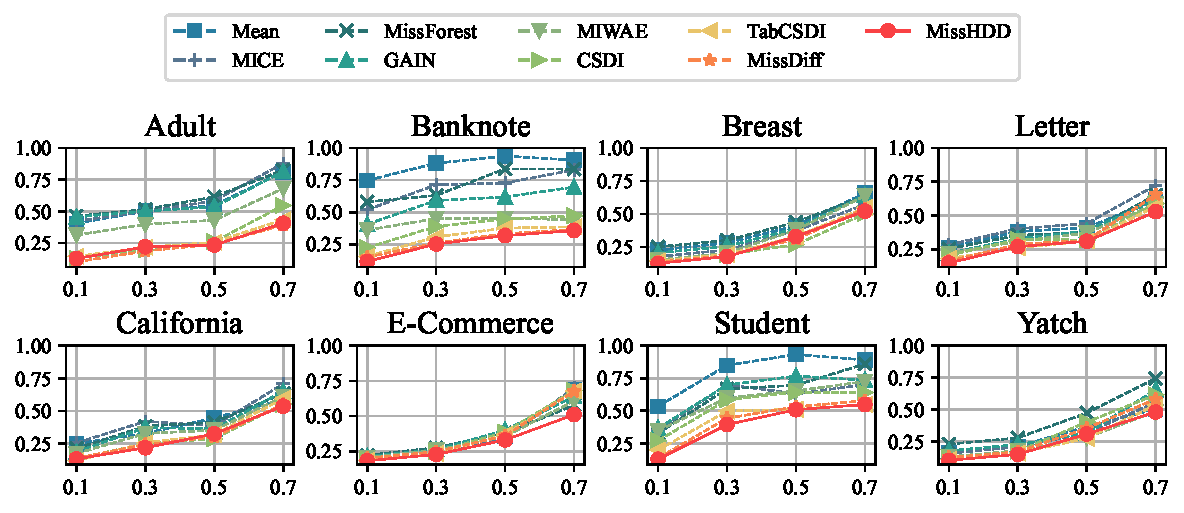
\includegraphics[width=\linewidth]{evaluate_mcar_grid}
        \caption{MCAR}
        \label{fig:rmse_mcar}
    \end{subfigure}
    \vspace{8pt}

    %---------------- MAR ----------------%
    \begin{subfigure}{0.9\linewidth}
        \centering
        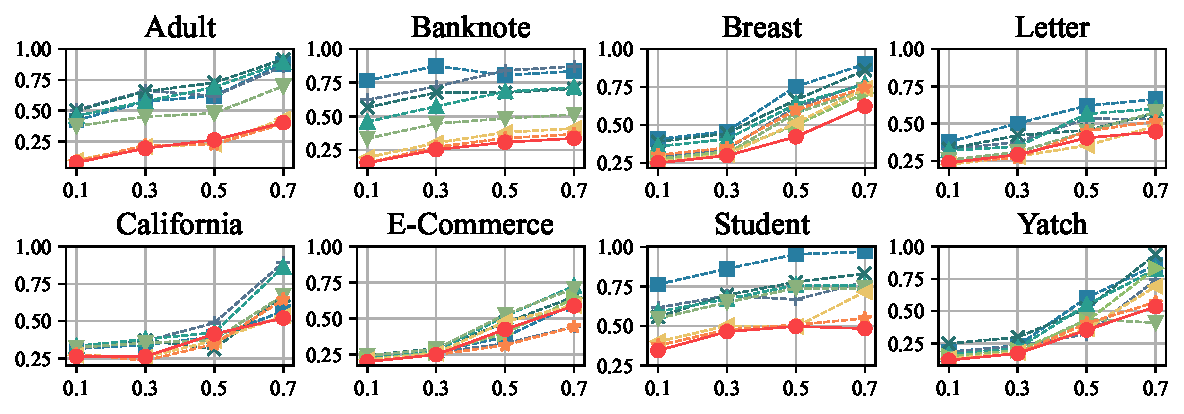
\includegraphics[width=\linewidth]{evaluate_mar_grid}
        \caption{MAR}
        \label{fig:rmse_mar}
    \end{subfigure}
    \vspace{8pt}

    %---------------- MNAR ----------------%
    \begin{subfigure}{0.9\linewidth}
        \centering
        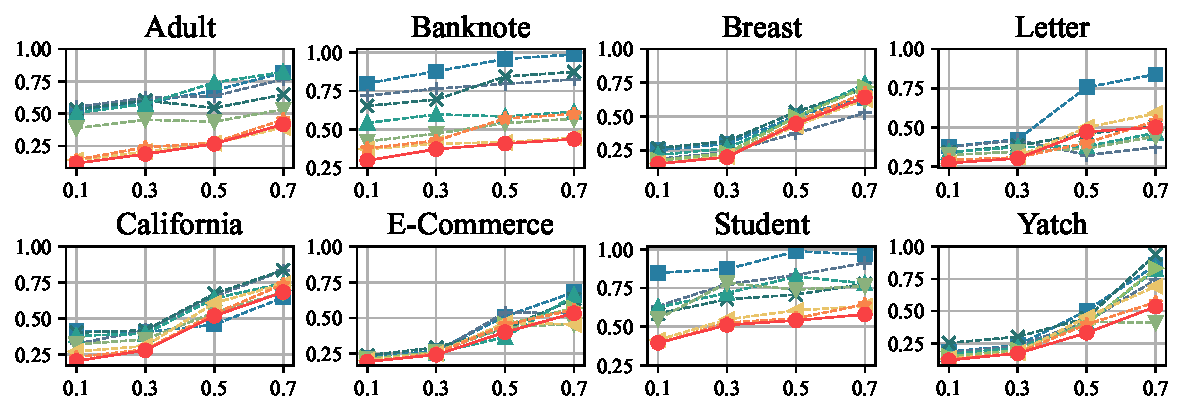
\includegraphics[width=\linewidth]{evaluate_mnar_grid}
        \caption{MNAR}
        \label{fig:rmse_mnar}
    \end{subfigure}

    \caption{
        Imputation accuracy under three missingness mechanisms: 
        \textbf{MCAR}, \textbf{MAR}, and \textbf{MNAR}.
    }
    \label{fig:rmse_missingness_all}
\end{figure*}

% \begin{figure*}[ht!]
%     \centering
    
%     %---------------- MCAR ----------------%
%     \begin{subfigure}{0.9\linewidth}
%         \centering
%         \includegraphics[width=\linewidth]{evaluate_mcar_grid_with_boxplot}
%         \caption{MCAR}
%         \label{fig:rmse_mcar}
%     \end{subfigure}
%     \vspace{8pt}

%     %---------------- MAR ----------------%
%     \begin{subfigure}{0.9\linewidth}
%         \centering
%         \includegraphics[width=\linewidth]{evaluate_mar_grid_with_boxplot}
%         \caption{MAR}
%         \label{fig:rmse_mar}
%     \end{subfigure}
%     \vspace{8pt}

%     %---------------- MNAR ----------------%
%     \begin{subfigure}{0.9\linewidth}
%         \centering
%         \includegraphics[width=\linewidth]{evaluate_mnar_grid_with_boxplot}
%         \caption{MNAR}
%         \label{fig:rmse_mnar}
%     \end{subfigure}

%     \caption{
%         Imputation accuracy under three missingness mechanisms: 
%         \textbf{MCAR}, \textbf{MAR}, and \textbf{MNAR}.
%         Each subplot displays dataset-wise ImpErr curves (left) and 
%         aggregated error distributions (right) across missing rates.
%     }
%     \label{fig:rmse_missingness_all}
% \end{figure*}



\section{Results and Analysis}



\subsection{Imputation Accuracy}
We evaluate imputation quality under \textbf{MCAR}, \textbf{MAR}, and
\textbf{MNAR} missingness at rates of 10\%, 30\%, 50\%, and 70\%.
Figures~\ref{fig:rmse_mcar}, \ref{fig:rmse_mar}, and~\ref{fig:rmse_mnar}
report ImpErr on fully observed datasets with synthetic masks, while
Figure~\ref{fig:miss_mechanism_boxplots} summarizes the aggregated
distributions.

ImpErr increases with missingness severity, especially under MAR and MNAR.
Classical and latent-variable baselines degrade more sharply, while diffusion
baselines remain sensitive to categorical features. \texttt{MissHDD} achieves
lower ImpErr across mechanisms and rates, with lower median error and smaller
variance in the aggregated boxplots.





\begin{figure}[t]
    \centering
    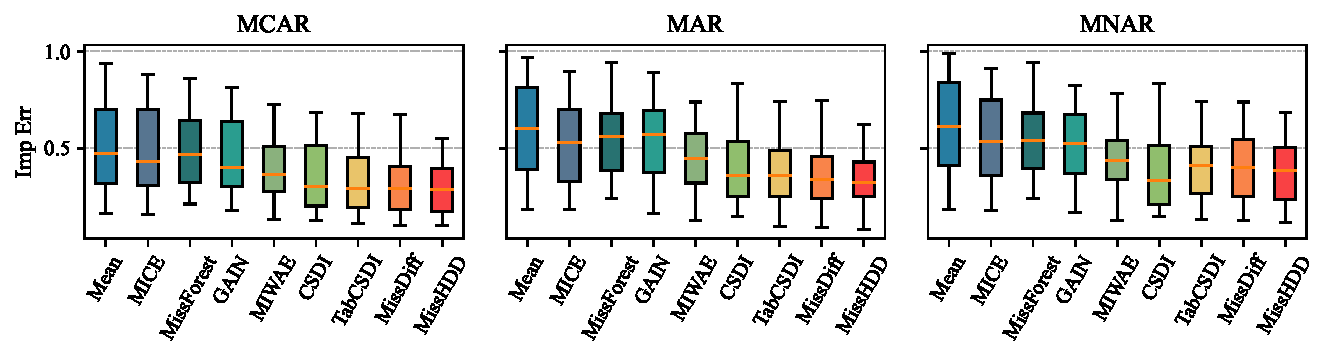
\includegraphics[width=1\linewidth]{evaluate_miss_mechanisms_boxplots.pdf}
    \caption{
        Aggregated imputation performance across all datasets under the 
        three missingness mechanisms: \textbf{MCAR}, \textbf{MAR}, and \textbf{MNAR}. 
        Each boxplot summarizes the distribution of ImpErr across missing rates 
        and datasets; lower values indicate better imputation quality.
    }
    \label{fig:miss_mechanism_boxplots}
\end{figure}


% Downstream F1
\begin{table*}[!t]
\centering
\caption{Category~1 classification F1~($\uparrow$), mean $\pm$ std. \best{Bold}
and \secondbest{underline} mark best and second-best scores.}
\label{tab:classification_results}
\resizebox{\textwidth}{!}{
\begin{tabular}{l|ccc|ccc|}
\hline
\textbf{Method}  & \multicolumn{3}{c|}{\textbf{Adult}} & \multicolumn{3}{c|}{\textbf{Banknote}} \\
\hline
\textbf{Rate} & 30\% & 50\% & 70\% & 30\% & 50\% & 70\% \\
\hline
Mean & \meanstd{0.4966}{0.0084} & \meanstd{0.4750}{0.0084} & \meanstd{0.4440}{0.0095} & \meanstd{0.9000}{0.0123} & \meanstd{0.7870}{0.0147} & \meanstd{0.6703}{0.0195} \\
MICE & \meanstd{0.6734}{0.0117} & \meanstd{0.6447}{0.0145} & \meanstd{0.6218}{0.0290} & \meanstd{0.9416}{0.0104} & \meanstd{0.8414}{0.0133} & \meanstd{0.7512}{0.0126} \\
MissForest & \meanstd{0.6971}{0.0226} & \meanstd{0.6517}{0.0264} & \best{\meanstd{0.6347}{0.0264}} & \secondbest{\meanstd{0.9517}{0.0095}} & \meanstd{0.8727}{0.0103} & \meanstd{0.7821}{0.0128} \\
\hline
GAIN & \meanstd{0.6048}{0.0124} & \meanstd{0.5775}{0.0225} & \meanstd{0.5441}{0.0295} & \meanstd{0.9217}{0.0235} & \meanstd{0.8725}{0.0257} & \meanstd{0.7957}{0.0324} \\
MIWAE & \meanstd{0.6941}{0.0104} & \meanstd{0.6327}{0.0197} & \meanstd{0.6014}{0.0222} & \meanstd{0.9226}{0.0201} & \meanstd{0.8937}{0.0250} & \meanstd{0.8125}{0.0330} \\
\hline
CSDI & \meanstd{0.6827}{0.0127} & \meanstd{0.6424}{0.0134} & \meanstd{0.6218}{0.0172} & \meanstd{0.9358}{0.0159} & \meanstd{0.8867}{0.0251} & \meanstd{0.8025}{0.0297} \\
TabCSDI & \secondbest{\meanstd{0.7214}{0.0198}} & \best{\meanstd{0.6851}{0.0211}} & \secondbest{\meanstd{0.6318}{0.0224}} & \best{\meanstd{0.9527}{0.0126}} & \secondbest{\meanstd{0.9014}{0.0175}} & \secondbest{\meanstd{0.8657}{0.0214}} \\
MissDiff & \meanstd{0.7046}{0.0126} & \meanstd{0.6711}{0.0154} & \meanstd{0.6247}{0.0157} & \meanstd{0.9416}{0.1140} & \meanstd{0.8867}{0.1645} & \meanstd{0.8237}{0.0201} \\
MissHDD & \best{\meanstd{0.7228}{0.0104}} & \secondbest{\meanstd{0.6724}{0.0124}} & \secondbest{\meanstd{0.6318}{0.0145}} & \best{\meanstd{0.9527}{0.1240}} & \best{\meanstd{0.9214}{0.1470}} & \best{\meanstd{0.8772}{0.0195}} \\
\hline
\end{tabular}
}
\vspace{0.6em}
\resizebox{\textwidth}{!}{
\begin{tabular}{l|ccc|ccc|}
\hline
\textbf{Method}  & \multicolumn{3}{c|}{\textbf{Breast}} & \multicolumn{3}{c|}{\textbf{Letter}} \\
\hline
\textbf{Rate} & 30\% & 50\% & 70\% & 30\% & 50\% & 70\% \\
\hline
Mean & \meanstd{0.7632}{0.0007} & \meanstd{0.6628}{0.0011} & \meanstd{0.5119}{0.0014} & \meanstd{0.7960}{0.0004} & \meanstd{0.6277}{0.0017} & \meanstd{0.4046}{0.0022} \\
MICE & \meanstd{0.6906}{0.0006} & \meanstd{0.6301}{0.0012} & \meanstd{0.4932}{0.0018} & \meanstd{0.7862}{0.0002} & \meanstd{0.7850}{0.0007} & \meanstd{0.4370}{0.0012} \\
MissForest & \meanstd{0.7097}{0.0006} & \meanstd{0.6424}{0.0014} & \secondbest{\meanstd{0.5243}{0.0020}} & \meanstd{0.8323}{0.0004} & \meanstd{0.8148}{0.0007} & \meanstd{0.4524}{0.0011} \\
\hline
GAIN & \meanstd{0.7178}{0.0011} & \meanstd{0.6399}{0.0015} & \meanstd{0.4961}{0.0021} & \meanstd{0.8221}{0.0011} & \meanstd{0.7567}{0.0017} & \meanstd{0.4054}{0.0019} \\
MIWAE & \meanstd{0.7542}{0.0014} & \meanstd{0.5805}{0.0016} & \meanstd{0.5223}{0.0024} & \meanstd{0.8674}{0.0007} & \meanstd{0.8186}{0.0009} & \meanstd{0.4253}{0.0014} \\
\hline
CSDI & \meanstd{0.7305}{0.0009} & \meanstd{0.7030}{0.0011} & \meanstd{0.5177}{0.0019} & \meanstd{0.8479}{0.0009} & \meanstd{0.8090}{0.0014} & \meanstd{0.4249}{0.0018} \\
TabCSDI & \secondbest{\meanstd{0.7730}{0.0014}} & \meanstd{0.7278}{0.0017} & \best{\meanstd{0.5282}{0.0018}} & \secondbest{\meanstd{0.9049}{0.0014}} & \secondbest{\meanstd{0.8471}{0.0019}} & \meanstd{0.4467}{0.0022} \\
MissDiff & \meanstd{0.7445}{0.0011} & \secondbest{\meanstd{0.7293}{0.0016}} & \meanstd{0.5185}{0.0018} & \meanstd{0.8503}{0.0015} & \meanstd{0.8242}{0.0019} & \secondbest{\meanstd{0.4541}{0.0021}} \\
MissHDD & \best{\meanstd{0.7873}{0.0008}} & \best{\meanstd{0.7524}{0.0014}} & \meanstd{0.5202}{0.0017} & \best{\meanstd{0.9117}{0.0012}} & \best{\meanstd{0.8559}{0.0014}} & \best{\meanstd{0.4581}{0.0017}} \\
\hline
\end{tabular}
}
\end{table*}

% Downstream MAE
\begin{table*}[!t]
\centering
\caption{Category~1 regression MAE~($\downarrow$), mean $\pm$ std. \best{Bold}
and \secondbest{underline} mark best and second-best scores.}
\label{tab:regression_results}
\resizebox{\textwidth}{!}{
\begin{tabular}{l|ccc|ccc|}
\hline
\textbf{Method}  & \multicolumn{3}{c|}{\textbf{Yacht}} & \multicolumn{3}{c|}{\textbf{E-commerce}} \\
\hline
\textbf{Rate} & 30\% & 50\% & 70\% & 30\% & 50\% & 70\% \\
\hline
Mean & \meanstd{1.1748}{0.0124} & \meanstd{1.3966}{0.0119} & \meanstd{1.5177}{0.0123} & \meanstd{1.1264}{0.0124} & \meanstd{1.2585}{0.0147} & \meanstd{1.3947}{0.0155} \\
MICE & \meanstd{1.3032}{0.0114} & \meanstd{1.2830}{0.0104} & \meanstd{1.5076}{0.0117} & \meanstd{1.2040}{0.0135} & \meanstd{1.2180}{0.0157} & \meanstd{1.4373}{0.0158} \\
MissForest & \meanstd{1.3681}{0.0248} & \meanstd{1.3306}{0.0255} & \meanstd{1.6776}{0.0201} & \meanstd{1.2887}{0.0147} & \meanstd{1.2245}{0.0142} & \meanstd{1.5723}{0.0159} \\
\hline
GAIN & \meanstd{1.0437}{0.0234} & \meanstd{1.2341}{0.0215} & \meanstd{1.3778}{0.0214} & \meanstd{0.9787}{0.0155} & \meanstd{1.1108}{0.0124} & \meanstd{1.2736}{0.0164} \\
MIWAE & \meanstd{1.0460}{0.0184} & \meanstd{1.2262}{0.0177} & \meanstd{1.2757}{0.0175} & \meanstd{0.9245}{0.0164} & \meanstd{1.1464}{0.0145} & \meanstd{1.1795}{0.0165} \\
\hline
CSDI & \meanstd{0.8049}{0.0241} & \meanstd{1.0274}{0.0207} & \meanstd{1.0349}{0.0195} & \meanstd{0.7296}{0.0145} & \meanstd{0.9554}{0.0136} & \meanstd{0.8932}{0.0149} \\
TabCSDI & \secondbest{\meanstd{0.6397}{0.0201}} & \best{\meanstd{0.9127}{0.0211}} & \meanstd{0.9578}{0.0204} & \best{\meanstd{0.5238}{0.0156}} & \secondbest{\meanstd{0.8379}{0.0146}} & \secondbest{\meanstd{0.8614}{0.0155}} \\
MissDiff & \meanstd{0.7099}{0.0145} & \meanstd{0.9346}{0.0095} & \secondbest{\meanstd{0.9477}{0.0114}} & \meanstd{0.5748}{0.0147} & \meanstd{0.8508}{0.0128} & \best{\meanstd{0.8591}{0.0133}} \\
MissHDD & \best{\meanstd{0.5668}{0.0125}} & \secondbest{\meanstd{0.9313}{0.0102}} & \best{\meanstd{0.9203}{0.0124}} & \secondbest{\meanstd{0.5260}{0.0149}} & \best{\meanstd{0.8054}{0.0145}} & \meanstd{0.8641}{0.0157} \\
\hline
\end{tabular}
}
\vspace{0.6em}
\resizebox{\textwidth}{!}{
\begin{tabular}{l|ccc|ccc|}
\hline
\textbf{Method}  & \multicolumn{3}{c|}{\textbf{California}} & \multicolumn{3}{c|}{\textbf{Student}} \\
\hline
\textbf{Rate} & 30\% & 50\% & 70\% & 30\% & 50\% & 70\% \\
\hline
Mean & \meanstd{0.5310}{0.0014} & \meanstd{0.6547}{0.0021} & \meanstd{0.7193}{0.0024} & \meanstd{2.2286}{0.0247} & \meanstd{2.3608}{0.0214} & \meanstd{2.5107}{0.0253} \\
MICE & \secondbest{\meanstd{0.5009}{0.0014}} & \meanstd{0.6439}{0.0015} & \meanstd{0.7241}{0.0021} & \meanstd{2.0147}{0.0231} & \meanstd{2.1097}{0.0255} & \meanstd{2.4936}{0.0244} \\
MissForest & \meanstd{0.5098}{0.0016} & \best{\meanstd{0.5832}{0.0017}} & \meanstd{0.7519}{0.0023} & \meanstd{1.7569}{0.0247} & \meanstd{2.0165}{0.0215} & \meanstd{1.9655}{0.0236} \\
\hline
GAIN & \meanstd{0.5214}{0.0017} & \meanstd{0.7130}{0.0018} & \meanstd{0.7384}{0.0020} & \meanstd{1.2574}{0.0233} & \meanstd{1.4025}{0.0235} & \meanstd{1.5993}{0.0231} \\
MIWAE & \meanstd{0.5160}{0.0015} & \meanstd{0.7281}{0.0022} & \meanstd{0.7711}{0.0027} & \meanstd{1.2347}{0.0210} & \meanstd{1.4582}{0.0219} & \meanstd{1.4614}{0.0195} \\
\hline
CSDI & \meanstd{0.5191}{0.0012} & \meanstd{0.7085}{0.0021} & \meanstd{0.7463}{0.0020} & \meanstd{1.0257}{0.0188} & \meanstd{1.2477}{0.1950} & \meanstd{1.2098}{0.0201} \\
TabCSDI & \meanstd{0.5103}{0.0017} & \secondbest{\meanstd{0.6393}{0.0019}} & \secondbest{\meanstd{0.6908}{0.0018}} & \meanstd{0.8712}{0.0195} & \meanstd{1.1371}{0.0211} & \meanstd{1.1816}{0.0209} \\
MissDiff & \meanstd{0.5242}{0.0015} & \meanstd{0.6565}{0.0016} & \meanstd{0.7481}{0.0021} & \secondbest{\meanstd{0.8571}{0.0162}} & \secondbest{\meanstd{1.1297}{0.0184}} & \best{\meanstd{1.1575}{0.0195}} \\
MissHDD & \best{\meanstd{0.4907}{0.0015}} & \meanstd{0.6422}{0.0018} & \best{\meanstd{0.6827}{0.0022}} & \best{\meanstd{0.8214}{0.0162}} & \best{\meanstd{1.1143}{0.0175}} & \secondbest{\meanstd{1.1713}{0.0194}} \\
\hline
\end{tabular}
}
\end{table*}

% Downstream Incomplete
\begin{table*}[!ht]
\centering
\caption{Category~2 Accuracy and NMI~($\uparrow$), mean $\pm$ std.
\best{Bold} and \secondbest{underline} mark best and second-best scores.}
\label{tab:incomplete_data}
\resizebox{\textwidth}{!}{
\begin{tabular}{lrrrrrr}
\toprule
\multirow{2}{*}{\textbf{Method}}  & \multicolumn{2}{c}{\textbf{Hepat}} & \multicolumn{2}{c}{\textbf{Horse}} & \multicolumn{2}{c}{\textbf{Kidney}} \\
\cmidrule(lr){2-3}\cmidrule(lr){4-5}\cmidrule(lr){6-7}
 & ACC & NMI & ACC & NMI & ACC & NMI \\
\midrule\midrule
Mean & \meanstd{0.8129}{0.0125} & \meanstd{0.0015}{0.0001} & \meanstd{0.8398}{0.0114} & \meanstd{0.0078}{0.0013} & \meanstd{0.9750}{0.0100} & \meanstd{0.0067}{0.0012} \\
MICE & \meanstd{0.8129}{0.0147} & \meanstd{0.0021}{0.0002} & \meanstd{0.8506}{0.0152} & \meanstd{0.0024}{0.0002} & \meanstd{0.9750}{0.0112} & \meanstd{0.0074}{0.0130} \\
MissForest & \meanstd{0.8065}{0.0133} & \meanstd{0.0014}{0.0003} & \meanstd{0.8262}{0.0147} & \meanstd{0.0078}{0.0006} & \meanstd{0.9650}{0.0142} & \meanstd{0.0023}{0.0070} \\
\midrule
GAIN & \secondbest{\meanstd{0.8274}{0.0145}} & \meanstd{0.0012}{0.0002} & \meanstd{0.8506}{0.0163} & \meanstd{0.0071}{0.0008} & \meanstd{0.8525}{0.0159} & \meanstd{0.0160}{0.0015} \\
MIWAE & \meanstd{0.8065}{0.0143} & \meanstd{0.0017}{0.0003} & \meanstd{0.8478}{0.0147} & \meanstd{0.0079}{0.0011} & \meanstd{0.8715}{0.0147} & \meanstd{0.0175}{0.0013} \\
\midrule
CSDI & \best{\meanstd{0.8367}{0.0185}} & \best{\meanstd{0.0814}{0.0140}} & \meanstd{0.8533}{0.0132} & \secondbest{\meanstd{0.0911}{0.0142}} & \meanstd{0.9825}{0.0132} & \meanstd{0.1234}{0.0068} \\
TabCSDI & \secondbest{\meanstd{0.8274}{0.0175}} & \secondbest{\meanstd{0.0809}{0.0110}} & \secondbest{\meanstd{0.8614}{0.0113}} & \meanstd{0.0883}{0.0114} & \best{\meanstd{0.9875}{0.0144}} & \secondbest{\meanstd{0.1531}{0.0057}} \\
MissDiff & \meanstd{0.8014}{0.0164} & \secondbest{\meanstd{0.0809}{0.0110}} & \meanstd{0.8451}{0.0126} & \meanstd{0.0611}{0.0095} & \secondbest{\meanstd{0.9850}{0.0157}} & \meanstd{0.0945}{0.0022} \\
MissHDD & \secondbest{\meanstd{0.8274}{0.0165}} & \secondbest{\meanstd{0.0809}{0.0110}} & \best{\meanstd{0.8641}{0.0158}} & \best{\meanstd{0.1025}{0.0074}} & \best{\meanstd{0.9875}{0.0124}} & \best{\meanstd{0.1714}{0.0047}} \\
\bottomrule
\end{tabular}
}
\vspace{0.6em}
\resizebox{\textwidth}{!}{
\begin{tabular}{lrrrrrr}
\toprule
\multirow{2}{*}{\textbf{Method}}  & \multicolumn{2}{c}{\textbf{Mammo}} & \multicolumn{2}{c}{\textbf{Pima}} & \multicolumn{2}{c}{\textbf{Wiscon}} \\
\cmidrule(lr){2-3}\cmidrule(lr){4-5}\cmidrule(lr){6-7}
 & ACC & NMI & ACC & NMI & ACC & NMI \\
\midrule\midrule
Mean & \meanstd{0.8148}{0.0125} & \meanstd{0.0959}{0.0147} & \meanstd{0.7735}{0.0114} & \meanstd{0.0111}{0.0124} & \meanstd{0.9628}{0.0124} & \meanstd{0.7295}{0.0214} \\
MICE & \meanstd{0.8241}{0.0147} & \meanstd{0.0959}{0.0147} & \meanstd{0.7722}{0.0131} & \meanstd{0.0910}{0.0114} & \meanstd{0.9614}{0.0136} & \best{\meanstd{0.7427}{0.0234}} \\
MissForest & \meanstd{0.8200}{0.0113} & \meanstd{0.0959}{0.0147} & \meanstd{0.7722}{0.0113} & \meanstd{0.0169}{0.0122} & \meanstd{0.9628}{0.0135} & \meanstd{0.7335}{0.0236} \\
\midrule
GAIN & \meanstd{0.8106}{0.0168} & \meanstd{0.0932}{0.0142} & \meanstd{0.7462}{0.0125} & \meanstd{0.0596}{0.0142} & \meanstd{0.9642}{0.0158} & \secondbest{\meanstd{0.7387}{0.0234}} \\
MIWAE & \meanstd{0.7971}{0.0188} & \meanstd{0.0841}{0.0112} & \meanstd{0.7786}{0.0185} & \meanstd{0.0621}{0.0116} & \meanstd{0.9521}{0.0149} & \meanstd{0.7017}{0.0208} \\
\midrule
CSDI & \secondbest{\meanstd{0.8292}{0.0169}} & \meanstd{0.1032}{0.0095} & \meanstd{0.8047}{0.0124} & \meanstd{0.1024}{0.0214} & \meanstd{0.9671}{0.0136} & \meanstd{0.7295}{0.0214} \\
TabCSDI & \best{\meanstd{0.8325}{0.0146}} & \secondbest{\meanstd{0.1124}{0.0132}} & \secondbest{\meanstd{0.8099}{0.0101}} & \secondbest{\meanstd{0.1124}{0.0195}} & \secondbest{\meanstd{0.9785}{0.0127}} & \meanstd{0.7335}{0.0217} \\
MissDiff & \meanstd{0.8179}{0.0133} & \meanstd{0.0945}{0.0145} & \best{\meanstd{0.8112}{0.0162}} & \meanstd{0.0750}{0.0124} & \meanstd{0.9671}{0.0115} & \meanstd{0.7038}{0.0299} \\
MissHDD & \best{\meanstd{0.8325}{0.0149}} & \best{\meanstd{0.1218}{0.0146}} & \secondbest{\meanstd{0.8099}{0.0143}} & \best{\meanstd{0.1321}{0.0010}} & \best{\meanstd{0.9871}{0.0136}} & \best{\meanstd{0.7427}{0.0215}} \\
\bottomrule
\end{tabular}
}
\end{table*}

\subsection{Downstream task utility}

We further evaluate whether imputed values preserve predictive structure.
Tables~\ref{tab:classification_results}--\ref{tab:incomplete_data} show that
MissHDD is frequently best or second-best on Category~1 and remains competitive
on the smaller naturally incomplete datasets.

\subsection{Statistical comparison}

We also perform a pooled rank-based comparison over all downstream evaluation
units: 12 F1, 12 MAE, six ACC, and six NMI units. Methods are ranked within
each unit by metric direction, and average ranks are compared using
\texttt{critdd} with Holm adjustment.

Figure~\ref{fig:cd_downstream} summarizes the pooled downstream ranking.
MissHDD obtains the best average rank, with TabCSDI as the closest competitor;
the metric-specific ranks follow the same trend.

\begin{figure}[!t]
\centering
\resizebox{0.92\textwidth}{!}{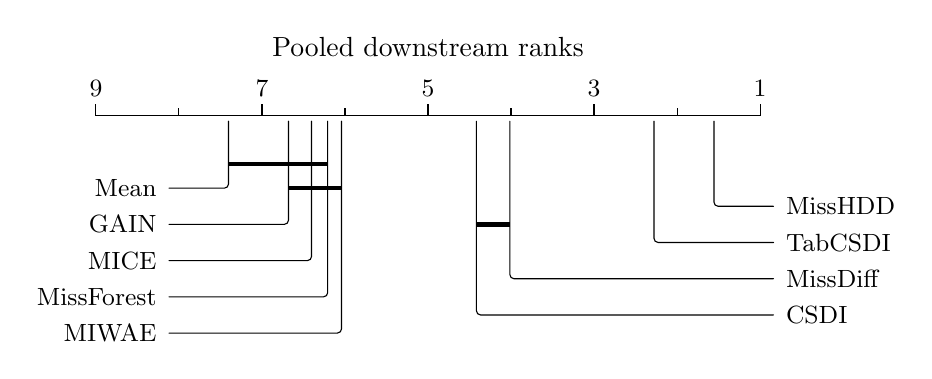
\begin{tikzpicture}[
  treatment line/.style={rounded corners=1.5pt, line cap=round, shorten >=1pt},
  treatment label/.style={font=\small},
  group line/.style={ultra thick},
]

\begin{axis}[
  clip={false},
  axis x line={center},
  axis y line={none},
  axis line style={-},
  xmin={1},
  ymax={0},
  scale only axis={true},
  width={\axisdefaultwidth},
  ticklabel style={anchor=south, yshift=1.3*\pgfkeysvalueof{/pgfplots/major tick length}, font=\small},
  every tick/.style={draw=black},
  major tick style={yshift=.5*\pgfkeysvalueof{/pgfplots/major tick length}},
  minor tick style={yshift=.5*\pgfkeysvalueof{/pgfplots/minor tick length}},
  title style={yshift=\baselineskip},
  xmax={9},
  ymin={-5.5},
  height={6\baselineskip},
  xtick={1,3,5,7,9},
  minor x tick num={1},
  x dir={reverse},
  title={Pooled downstream ranks},
]

\draw[treatment line] ([yshift=-2pt] axis cs:1.5555555555555556, 0) |- (axis cs:0.8055555555555556, -2.5)
  node[treatment label, anchor=west] {MissHDD};
\draw[treatment line] ([yshift=-2pt] axis cs:2.2777777777777777, 0) |- (axis cs:0.8055555555555556, -3.5)
  node[treatment label, anchor=west] {TabCSDI};
\draw[treatment line] ([yshift=-2pt] axis cs:4.013888888888889, 0) |- (axis cs:0.8055555555555556, -4.5)
  node[treatment label, anchor=west] {MissDiff};
\draw[treatment line] ([yshift=-2pt] axis cs:4.416666666666667, 0) |- (axis cs:0.8055555555555556, -5.5)
  node[treatment label, anchor=west] {CSDI};
\draw[treatment line] ([yshift=-2pt] axis cs:6.041666666666667, 0) |- (axis cs:8.152777777777779, -6.0)
  node[treatment label, anchor=east] {MIWAE};
\draw[treatment line] ([yshift=-2pt] axis cs:6.208333333333333, 0) |- (axis cs:8.152777777777779, -5.0)
  node[treatment label, anchor=east] {MissForest};
\draw[treatment line] ([yshift=-2pt] axis cs:6.402777777777778, 0) |- (axis cs:8.152777777777779, -4.0)
  node[treatment label, anchor=east] {MICE};
\draw[treatment line] ([yshift=-2pt] axis cs:6.680555555555555, 0) |- (axis cs:8.152777777777779, -3.0)
  node[treatment label, anchor=east] {GAIN};
\draw[treatment line] ([yshift=-2pt] axis cs:7.402777777777778, 0) |- (axis cs:8.152777777777779, -2.0)
  node[treatment label, anchor=east] {Mean};
\draw[group line] (axis cs:4.013888888888889, -3.0) -- (axis cs:4.416666666666667, -3.0);
\draw[group line] (axis cs:6.041666666666667, -2.0) -- (axis cs:6.680555555555555, -2.0);
\draw[group line] (axis cs:6.208333333333333, -1.3333333333333333) -- (axis cs:7.402777777777778, -1.3333333333333333);

\end{axis}
\end{tikzpicture}}
\caption{Pooled downstream critical-difference diagram. Lower rank is better;
bars indicate methods not separated by Holm adjustment at $\alpha=0.05$.}
\label{fig:cd_downstream}
\end{figure}





\subsection{Sampling Time}

CSDI, TabCSDI, and MissDiff use stochastic DDPM-style sampling, typically with
100 trajectories per instance. MissHDD uses a deterministic DDIM-like
trajectory, so one pass is sufficient. Since these baselines operate on
continuous features only, runtime is measured on numerical datasets using
MissHDD's continuous channel. Table~\ref{tab:inference_summary} compares the
standard 100-sample baseline protocol, a diagnostic one-sample baseline
protocol, and single-trajectory MissHDD with different diffusion lengths.
MissHDD achieves the lowest RMSE at $T{=}100$, while $T{=}50$ and $T{=}20$
trade small error increases for lower latency.
\begin{table}[!t]
\centering
\caption{
Inference time and RMSE~($\downarrow$). Baselines are reported under their
standard 100-sample stochastic protocol and a diagnostic one-sample protocol;
\texttt{MissHDD} uses one deterministic DDIM trajectory with varying $T$.
}
\label{tab:inference_summary}
\begin{tabular}{c|l|c|c}
\hline
\textbf{\#Samples} & \textbf{Method} 
& \textbf{Time (s) $\downarrow$}
& \textbf{RMSE $\downarrow$} \\
\hline
\multirow{3}{*}{100} 
& CSDI ($T{=}50$)      & 820.73 & 0.3730 \\
& TabCSDI ($T{=}50$)   & 794.21 & 0.3319 \\
& MissDiff ($T{=}50$)  & 765.92 & 0.3163 \\
\hline
\multirow{3}{*}{1} 
& CSDI ($T{=}50$)      & 435.20 & 0.4212 \\
& TabCSDI ($T{=}50$)   & 412.04 & 0.3752 \\
& MissDiff ($T{=}50$)  & 401.61 & 0.3125 \\
\hline
\multirow{3}{*}{1} 
& MissHDD ($T{=}100$) & 775.31 & \textbf{0.3051} \\
& MissHDD ($T{=}50$)  & 385.12 & 0.3167 \\
& MissHDD ($T{=}20$)  & \textbf{154.61} & 0.3343 \\
\hline
\end{tabular}
\end{table}








\section{Ablation Study}


\subsection{Synthetic heterogeneous dataset for ablation}

To isolate component contributions, we construct a controlled synthetic
heterogeneous dataset with $10{,}000$ samples and 30 features: 15 continuous
and 15 categorical.

Both feature types are generated from a shared latent Gaussian vector, inducing
nonlinear cross-type dependencies. Continuous features use smooth nonlinear
transformations with Gaussian noise, while categorical features are sampled
from softmax logits derived from the same latent vector. Missing values are
then introduced under MCAR, MAR, and MNAR at 30\% and 50\% missingness.



% \subsection{Synthetic heterogeneous dataset for ablation}

% For this ablation study, we construct a synthetic
% heterogeneous tabular dataset where both the data-generating process and the
% missingness mechanisms are fully controlled.

% We generate $n = 10{,}000$ samples with $d = 30$ features, split into
% $d_{\mathrm{cont}} = 15$ continuous variables and $d_{\mathrm{cat}} = 15$
% categorical variables. Let $\mathbf{z} \in \mathbb{R}^{15}$ denote a latent
% Gaussian vector sampled as
% \[
% \mathbf{z} \sim \mathcal{N}(\mathbf{0}, \mathbf{I}_{15}).
% \]

% \paragraph{Continuous features.}
% Each continuous feature is generated as a nonlinear transformation of
% $\mathbf{z}$ with added Gaussian noise:
% \[
% x^{\mathrm{cont}}_k
% = \mathbf{a}_k^\top \mathbf{z}
%   + b_k \,\phi(\mathbf{c}_k^\top \mathbf{z})
%   + \varepsilon_k,
% \qquad
% \varepsilon_k \sim \mathcal{N}(0, \sigma^2),
% \]
% for $k = 1,\dots,d_{\mathrm{cont}}$, where
% $\phi(\cdot)$ is a smooth nonlinearity (e.g., $\tanh$),
% and $\mathbf{a}_k, \mathbf{c}_k \in \mathbb{R}^4$, $b_k \in \mathbb{R}$ and
% $\sigma > 0$ are fixed coefficients. This construction induces correlated,
% non-Gaussian continuous features, mimicking realistic tabular structure.

% \paragraph{Categorical features.}
% Each categorical feature $x^{\mathrm{cat}}_j$ takes values in
% $\{1,\dots,K_j\}$ with $K_j \in \{3,4,5\}$.
% We first compute class logits as linear functions of the shared latent vector:
% \[
% \boldsymbol{\ell}_j = W_j \mathbf{z} + \boldsymbol{\xi}_j,
% \qquad
% \boldsymbol{\xi}_j \sim \mathcal{N}(\mathbf{0}, \sigma_{\text{cat}}^2 \mathbf{I}),
% \]
% where $W_j \in \mathbb{R}^{K_j \times 4}$.
% Class probabilities are obtained via a softmax,
% $\boldsymbol{\pi}_j = \mathrm{softmax}(\boldsymbol{\ell}_j)$, and the
% categorical outcome is sampled as
% \[
% x^{\mathrm{cat}}_j \sim \mathrm{Cat}(\boldsymbol{\pi}_j),
% \qquad j = 1,\dots,d_{\mathrm{cat}}.
% \]
% This yields categorical variables that are strongly but nonlinearly
% correlated with the continuous ones through the shared latent vector
% $\mathbf{z}$.

% \paragraph{Missingness mechanisms}
% Starting from the fully observed synthetic dataset $\mathbf{X}$, we generate
% missingness masks $\mathbf{M}$ under the three canonical mechanisms
% (MCAR, MAR, MNAR) at target missing rates
% $\rho \in \{0.3, 0.5\}$:
% \begin{itemize}
%     \item \textbf{MCAR:} each entry is independently set to missing with
%     probability $\rho$, independent of all feature values.
%     \item \textbf{MAR:} for each feature $v$, the missingness probability
%     depends on another observed feature $u$
%     (e.g., larger values of $u$ induce a higher missing probability for $v$),
%     following the threshold-based construction used in our real-data
%     experiments.
%     \item \textbf{MNAR:} missingness depends on the value of the feature itself:
%     for continuous variables, extreme values (e.g., top/bottom quantiles) are
%     removed with higher probability; for categorical variables, a subset of
%     categories is assigned elevated missingness probability until the target
%     rate $\rho$ is reached.
% \end{itemize}

\subsection{Contribution of the Two-Channel Architecture}


\begin{table}[!t]
\centering
\caption{Two-channel ablation at 30\% and 70\% missingness under MCAR, MAR,
and MNAR.
The evaluation metric is \textbf{ImpErr}:  
for continuous-only settings it reduces to RMSE,  
and for categorical-only settings it reduces to classification error.}

\label{tab:ablation_two_channel}
\resizebox{0.80\textwidth}{!}{%
\begin{tabular}{l l c c c}
\toprule
Dataset & Model 
& MCAR-ImpErr $\downarrow$ 
& MAR-ImpErr $\downarrow$ 
& MNAR-ImpErr $\downarrow$ \\
\midrule
\multirow{3}{*}{Adult (30\%)} 
& DDIM-only  & 0.2345 & 0.2323 & 0.2523 \\
& LPDD-only  & 0.2574 & 0.3214 & 0.3124 \\
& \textbf{Full} & \best{0.2202} & \best{0.1956} & \best{0.1864} \\
\midrule
\multirow{3}{*}{Adult (70\%)} 
& DDIM-only  & 0.4312 & 0.4314 & 0.4552 \\
& LPDD-only  & 0.4712 & 0.5027 & 0.5632 \\
& \textbf{Full} & \best{0.4063} & \best{0.4029} & \best{0.4167} \\
\midrule
\multirow{3}{*}{Synthetic (30\%)} 
& DDIM-only  & 0.3837 & 0.3758 & 0.4248 \\
& LPDD-only  & 0.4521 & 0.4693 & 0.4851 \\
& \textbf{Full} & \best{0.3459} & \best{0.3581} & \best{0.3948} \\
\midrule
\multirow{3}{*}{Synthetic (70\%)} 
& DDIM-only  & 0.6421 & 0.7047 & 0.7623 \\
& LPDD-only  & 0.6821 & 0.7948 & 0.8124 \\
& \textbf{Full} & \best{0.5821} & \best{0.6471} & \best{0.7123} \\
\bottomrule
\end{tabular}}
\end{table}

We compare the full model with two single-channel variants: a continuous-only
DDIM model using numerical encodings for all features, and a discrete-only
LPDD model that discretises continuous features into quantile bins. The full
model consistently achieves lower imputation error. The continuous-only
variant suffers on categorical variables due to semantic drift, whereas the
discrete-only variant loses numerical precision through discretisation. This
supports the use of separate but coordinated generative mechanisms for
mixed-type data.

\subsection{Self-mask ratio and effectiveness}



\begin{table}[!t]
\centering
\caption{Self-masking ablation on the synthetic dataset with 50\% MCAR
missingness. Zero-Imp and Mean-Imp use no additional masking.}
\label{tab:ablation_self_mask}
\resizebox{0.8\textwidth}{!}{
\begin{tabular}{c l c c c}
\toprule
\textbf{Self-mask Strategy} 
& Ratio
& \textbf{MCAR-ImpErr $\downarrow$}
& \textbf{MAR-ImpErr $\downarrow$}
& \textbf{MNAR-ImpErr $\downarrow$} \\
\midrule

\multirow{2}{*}{\textbf{No Self-mask}} 
& Zero-Imp & 0.4231 & 0.4528 & 0.4612 \\
& Mean-Imp & 0.3545 & 0.3681 & 0.4048\\
\midrule

\multirow{3}{*}{\textbf{MCAR Self-mask}} 
& 10\%  & 0.3634 & 0.3728 & 0.4124 \\
& 30\%  & \best{0.3459} & 0.3581 & 0.3948 \\
& 50\%  & \best{0.3459} & \best{0.3501} & \best{0.3930} \\
\midrule

\multirow{3}{*}{\textbf{MAR Self-mask}} 
& 10\%  & 0.3759 & 0.3874 & 0.3852 \\
& 30\%  & \best{0.3532} & \best{0.3524} & \best{0.3749}\\
& 50\%  & 0.3592 & 0.3651 & 0.3824\\
\midrule

\multirow{3}{*}{\textbf{MNAR Self-mask}} 
& 10\%  & 0.3682 & 0.3839 & 0.4029\\
& 30\%  & \best{0.3524} & \best{0.3624} & 0.3849\\
& 50\%  & 0.3759 & 0.3749 & \best{0.3833}\\
\bottomrule
\end{tabular}}
\end{table}
Table~\ref{tab:ablation_self_mask} shows that auxiliary self-masking improves
ImpErr, with 30\% giving the most stable trade-off. No self-mask mechanism
dominates, so MCAR self-masking is a simple default.

% Table \ref{tab:ablation_self_mask} presents a detailed ablation of our self-masking design.
% We compare training without any auxiliary masking (“Zero-Imp” and “Mean-Imp”) against various self-masking ratios $(10\%, 30\%, 50\%)$ applied under MCAR, MAR, and MNAR masking schemes.

% First, models trained without self-masking exhibit the weakest performance across all three missingness mechanisms. This confirms that relying solely on the original mask causes the model to overfit specific missingness patterns and generalise poorly to unseen masks—particularly evident under MAR and MNAR, where the distribution shift between train-time and test-time masks is substantial.

% Introducing self-masking consistently improves ImpErr across all settings.
% Among all ratios, $30\%$ self-masking yields the most stable and competitive performance, striking a balance between providing sufficient pseudo-missing supervision and avoiding excessive corruption of observed features.
% Although $50\%$ masking can achieve comparable or slightly better results in some cases, we observe slower convergence and higher optimisation variance due to the reduced amount of intact conditioning information—an effect amplified on small synthetic datasets.
% Conversely, $10\%$ masking is generally insufficient: the model sees too few pseudo-missing entries to learn robust conditional distributions.

% Comparing different masking mechanisms (MCAR-, MAR-, MNAR-style self-masking), we observe no consistently dominant masking strategy across the evaluated settings. While MAR/MNAR masking occasionally offer small gains, the differences are marginal. For simplicity and robustness, MCAR-style self-masking emerges as the most reliable and computationally convenient choice, providing strong and consistent performance across all test mechanisms.

% Overall, these results demonstrate that self-masking is an essential component of our training pipeline: it improves robustness, stabilises training, and yields consistently lower errors without requiring additional clean data.


\subsection{Effect of Sampling Stochasticity and Diffusion Steps}


\begin{table}[!t]
\centering
\caption{
Impact of sampling stochasticity ($\eta$) and number of sampling steps ($T$)
on RMSE under 50\% missing rate. Lower is better.
}
\label{tab:eta_step_table}
\resizebox{\linewidth}{!}{
\begin{tabular}{c|cc|cc|cc|cc|cc}
\toprule
\multirow{2}{*}{$\eta$} 
& \multicolumn{2}{c|}{\textbf{Letter}}  
& \multicolumn{2}{c|}{\textbf{California}}  
& \multicolumn{2}{c|}{\textbf{Adult}}
& \multicolumn{2}{c|}{\textbf{Banknote}}
& \multicolumn{2}{c}{\textbf{Student}} \\

\cmidrule(lr){2-3}
\cmidrule(lr){4-5}
\cmidrule(lr){6-7}
\cmidrule(lr){8-9}
\cmidrule(lr){10-11}

& $T{=}25$ & $T{=}100$
& $T{=}25$ & $T{=}100$
& $T{=}25$ & $T{=}100$
& $T{=}25$ & $T{=}100$
& $T{=}25$ & $T{=}100$ \\
\midrule

0.0 
& \best{0.3214} & 0.2254
& \best{0.5014} & 0.3254
& \best{0.5014} & 0.2843
& \best{0.5322} & 0.3254
& \best{0.6322} & \best{0.5109} \\

0.5 
& 0.6780 & \best{0.2054}
& 0.7421 & 0.3054
& 0.6021 & 0.3142
& 0.8421 & 0.3017
& 0.8421 & 0.5119 \\

1.0 
& 0.7510 & 0.2796
& 0.8510 & \best{0.2996}
& 0.6412 & \best{0.2568}
& 0.8451 & \best{0.2966}
& 0.9210 & \best{0.5109} \\
\bottomrule
\end{tabular}
}
\end{table}


% \begin{table}[!t]
% \centering
% \caption{Impact of sampling stochasticity ($\eta$) and number of sampling steps ($T$) on RMSE under 50\% missing rate.
% %Lower values are better.
% }
% \label{tab:eta_step_table}
% \begin{tabular}{c|cc|cc|cc|cc|cc}
% \hline
% \multirow{2}{*}{$\eta$} & \multicolumn{2}{c|}{\textbf{Letter}} & \multicolumn{2}{c|}{\textbf{California}} & \multicolumn{2}{c}{\textbf{Adult}}& \multicolumn{2}{c}{\textbf{Banknote}}& \multicolumn{2}{c}{\textbf{Student}} \\
% \cline{2-7}
%  & 25  & 100 & 25  & 100 & 25  & 100 \\
% \hline
% 0.0 & \textbf{0.3214}  & 0.2254 & \textbf{0.5014}  & 0.3254 &\textbf{0.4977} & 0.3293\\
% 0.5 & 0.6780  & \textbf{0.2054} & 0.7421  & 0.3054 &0.7412  & \textbf{0.3167}\\
% 1.0 & 0.7510  & 0.2796 & 0.8510  & \textbf{0.2996} &0.8170 & 0.3343\\
% \hline
% \end{tabular}
% \end{table}


\begin{figure}[!h]
\centering
\begin{subfigure}[b]{0.325\columnwidth}
    \centering
    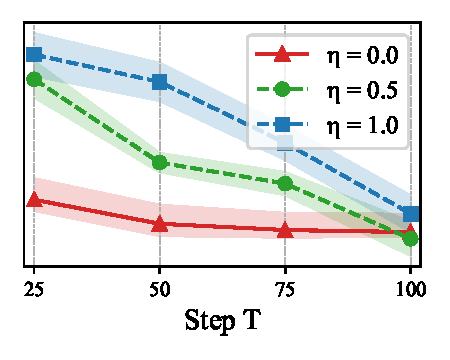
\includegraphics[width=\linewidth]{eval_var_T_letter.pdf}
    \vspace{-2em}
    \caption{Letter}
    \label{fig:ablation_sampling_letter}
\end{subfigure}
\hspace{-0.5em}
\begin{subfigure}[b]{0.325\columnwidth}
    \centering
    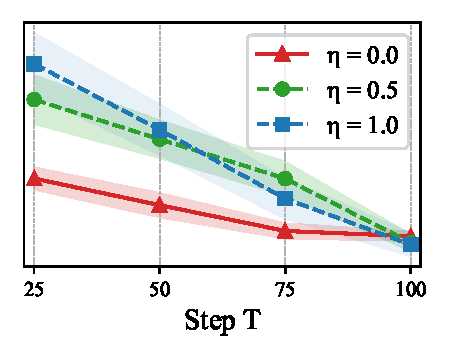
\includegraphics[width=\linewidth]{eval_var_T_cali.pdf}
            \vspace{-2em}
    \caption{California}
    \label{fig:ablation_sampling_cali}
\end{subfigure}
\hspace{-0.5em}
\begin{subfigure}[b]{0.325\columnwidth}
    \centering
    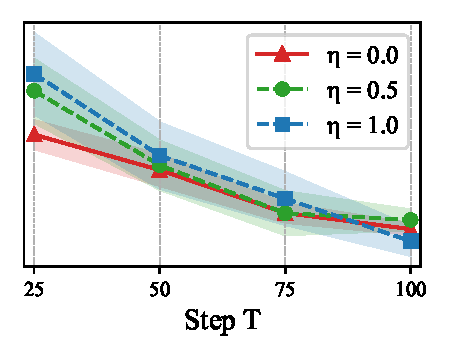
\includegraphics[width=\linewidth]{eval_var_T_adult.pdf}
            \vspace{-2em}
    \caption{Adult}
    \label{fig:ablation_sampling_adult}
\end{subfigure}
%\vspace{-0.5em} % Optional: reduce space before caption
\begin{subfigure}[b]{0.325\columnwidth}
    \centering
    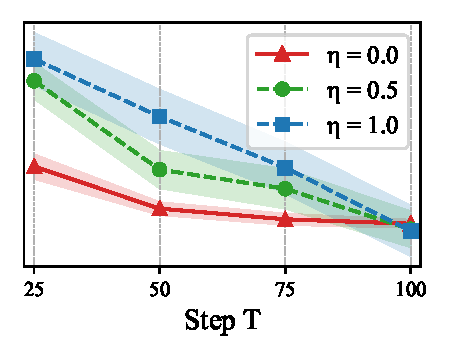
\includegraphics[width=\linewidth]{eval_var_T_bank.pdf}
            %\vspace{-2em}
    \caption{Banknote}
    \label{fig:ablation_sampling_bank}
\end{subfigure}
%\hspace{-0.5em}
\begin{subfigure}[b]{0.325\columnwidth}
    \centering
    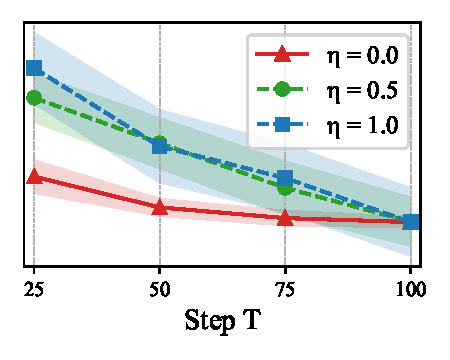
\includegraphics[width=\linewidth]{eval_var_T_student.pdf}
            %\vspace{-2em}
    \caption{Student}
    \label{fig:ablation_sampling_student}
\end{subfigure}
%\hspace{-0.5em}
\begin{subfigure}[b]{0.325\columnwidth}
    \centering
    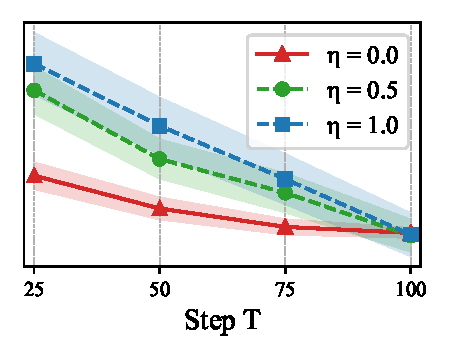
\includegraphics[width=\linewidth]{eval_var_T_avg.pdf}
            %\vspace{-2em}
    \caption{Average}
    \label{fig:ablation_sampling_avg}
\end{subfigure}
%\vspace{-0.5em}
%\caption{RMSE Comparing different sampling strategies under varying $\eta$ values.}
\caption{RMSE comparison with varying $\eta$ values.}
\label{fig:ablation_sampling_combined}
\end{figure}



To characterise the continuous diffusion channel, we vary DDIM stochasticity
$\eta \in \{0.0, 0.5, 1.0\}$ and the number of reverse steps
$T \in \{25, 50, 75, 100\}$. Here $\eta{=}0$ is deterministic and larger
values approach stochastic DDPM sampling, with injected variance
$
\sigma_{\tau_i}(\eta)
= \eta 
\sqrt{\frac{1 - \alpha_{\tau_{i-1}}}{1 - \alpha_{\tau_i}}}
\sqrt{1 - \frac{\alpha_{\tau_i}}{\alpha_{\tau_{i-1}}}},
$
without changing model parameters. The ablation results in
Table~\ref{tab:eta_step_table} and Figure~\ref{fig:ablation_sampling_combined}
show that $\eta{=}0$ gives low
variance and competitive accuracy, especially for small $T$. Stochastic
sampling can slightly improve some large-$T$ cases, but increases variance and
runtime, supporting the deterministic DDIM design used in MissHDD.

\section{Limitations}

Several limitations remain. First, LPDD provides simplex invariance and
empirical stability, but we do not prove convergence or probabilistic
consistency for the latent-path reverse dynamics. Second, MissHDD targets
stable point imputation and does not directly quantify uncertainty over
multiple plausible imputations. Third, the feature-wise simplex representation
scales with the total categorical vocabulary size \(\sum_j K_j\), so
high-cardinality variables may require shared embeddings, low-rank heads, or
top-$k$ truncation. Finally, self-masking depends on how well auxiliary masks
match test-time missingness.

\section{Conclusion}

We introduced \textbf{MissHDD}, a hybrid diffusion framework for incomplete
heterogeneous tabular data. By pairing deterministic DDIM updates for
continuous variables with LPDD-style simplex updates for categorical variables,
MissHDD models each feature type on its native domain while sharing observed
context across channels. Experiments across missingness mechanisms, missing
rates, and downstream tasks show improved accuracy, stability, and inference
efficiency over representative baselines.

Future work will extend MissHDD toward uncertainty-aware deterministic
ensembles, scalable high-cardinality categorical updates, ordinal variables,
and adaptive self-masking.



\section*{Acknowledgement}

This article is an extended version of our short paper accepted at the ACM International Conference on Information and Knowledge Management (CIKM) 2025 \cite{missddim}. In the CIKM short paper, we presented the {\tt MissDDIM} framework for imputing only numeric/continuous missing values. In this journal article, we extended the idea to impute both categorical and discrete missing values and introduced an integrated framework, {\tt MissHDD}, to impute missing values in incomplete heterogeneous tabular data. To cover the broader scope, we made substantial changes in all sections of the paper.     
This work is supported by the Air Force Office of Scientific Research under award number FA2386-23-1-4003 and Deakin University.

\section*{Declaration of generative AI and AI-assisted technologies in the manuscript}
During the preparation of this work, the author(s) used ChatGPT for minor language polishing to improve clarity and professional expression. After using this tool, the author(s) thoroughly reviewed and edited the content and take full responsibility for the final manuscript.

\bibliographystyle{elsarticle-num}
\bibliography{mybib}
\end{document}

\endinput
%%
%% End of file `elsarticle-template-num.tex'.
}
% % %% Use \section commands to start a section
% % \section{Example Section}
% % \label{sec1}
% % %% Labels are used to cross-reference an item using \ref command.

% % Section text. See Subsection \ref{subsec1}.

% % %% Use \subsection commands to start a subsection.
% % \subsection{Example Subsection}
% % \label{subsec1}


% % Subsection text.

% % %% Use \subsubsection, \paragraph, \subparagraph commands to 
% % %% start 3rd, 4th and 5th level sections.
% % %% Refer following link for more details.
% % %% https://en.wikibooks.org/wiki/LaTeX/Document_Structure#Sectioning_commands

% % \subsubsection{Mathematics}
% % %% Inline mathematics is tagged between $ symbols.
% % This is an example for the symbol $\alpha$ tagged as inline mathematics.

% % %% Displayed equations can be tagged using various environments. 
% % %% Single line equations can be tagged using the equation environment.
% % \begin{equation}
% % f(x) = (x+a)(x+b)
% % \end{equation}

% % %% Unnumbered equations are tagged using starred versions of the environment.
% % %% amsmath package needs to be loaded for the starred version of equation environment.
% % \begin{equation*}
% % f(x) = (x+a)(x+b)
% % \end{equation*}

% % %% align or eqnarray environments can be used for multi line equations.
% % %% & is used to mark alignment points in equations.
% % %% \\ is used to end a row in a multiline equation.
% % \begin{align}
% %  f(x) &= (x+a)(x+b) \\
% %       &= x^2 + (a+b)x + ab
% % \end{align}

% % \begin{eqnarray}
% %  f(x) &=& (x+a)(x+b) \nonumber\\ %% If equation numbering is not needed for a row use \nonumber.
% %       &=& x^2 + (a+b)x + ab
% % \end{eqnarray}

% % %% Unnumbered versions of align and eqnarray
% % \begin{align*}
% %  f(x) &= (x+a)(x+b) \\
% %       &= x^2 + (a+b)x + ab
% % \end{align*}

% % \begin{eqnarray*}
% %  f(x)&=& (x+a)(x+b) \\
% %      &=& x^2 + (a+b)x + ab
% % \end{eqnarray*}

% % %% Refer following link for more details.
% % %% https://en.wikibooks.org/wiki/LaTeX/Mathematics
% % %% https://en.wikibooks.org/wiki/LaTeX/Advanced_Mathematics

% % %% Use a table environment to create tables.
% % %% Refer following link for more details.
% % %% https://en.wikibooks.org/wiki/LaTeX/Tables
% % \begin{table}[t]%% placement specifier
% % %% Use tabular environment to tag the tabular data.
% % %% https://en.wikibooks.org/wiki/LaTeX/Tables#The_tabular_environment
% % \centering%% For centre alignment of tabular.
% % \begin{tabular}{l c r}%% Table column specifiers
% % %% Tabular cells are separated by &
% %   1 & 2 & 3 \\ %% A tabular row ends with \\
% %   4 & 5 & 6 \\
% %   7 & 8 & 9 \\
% % \end{tabular}
% % %% Use \caption command for table caption and label.
% % \caption{Table Caption}\label{fig1}
% % \end{table}


% % %% Use figure environment to create figures
% % %% Refer following link for more details.
% % %% https://en.wikibooks.org/wiki/LaTeX/Floats,_Figures_and_Captions
% % \begin{figure}[t]%% placement specifier
% % %% Use \includegraphics command to insert graphic files. Place graphics files in 
% % %% working directory.
% % \centering%% For centre alignment of image.
% % \includegraphics{example-image-a}
% % %% Use \caption command for figure caption and label.
% % \caption{Figure Caption}\label{fig1}
% % %% https://en.wikibooks.org/wiki/LaTeX/Importing_Graphics#Importing_external_graphics
% % \end{figure}


% % %% The Appendices part is started with the command \appendix;
% % %% appendix sections are then done as normal sections
% % \appendix
% % \section{Example Appendix Section}
% % \label{app1}

% % Appendix text.

% % %% For citations use: 
% % %%       \cite{<label>} ==> [1]

% % %%
% % Example citation, See \cite{lamport94}.

% % %% If you have bib database file and want bibtex to generate the
% % %% bibitems, please use
% % %%
% % %%  \bibliographystyle{elsarticle-num} 
% % %%  \bibliography{<your bibdatabase>}

% % %% else use the following coding to input the bibitems directly in the
% % %% TeX file.

% % %% Refer following link for more details about bibliography and citations.
% % %% https://en.wikibooks.org/wiki/LaTeX/Bibliography_Management
